% Options for packages loaded elsewhere
\PassOptionsToPackage{unicode}{hyperref}
\PassOptionsToPackage{hyphens}{url}
\PassOptionsToPackage{dvipsnames,svgnames,x11names}{xcolor}
%
\documentclass[
  letterpaper,
  DIV=11,
  numbers=noendperiod]{scrartcl}

\usepackage{amsmath,amssymb}
\usepackage{iftex}
\ifPDFTeX
  \usepackage[T1]{fontenc}
  \usepackage[utf8]{inputenc}
  \usepackage{textcomp} % provide euro and other symbols
\else % if luatex or xetex
  \usepackage{unicode-math}
  \defaultfontfeatures{Scale=MatchLowercase}
  \defaultfontfeatures[\rmfamily]{Ligatures=TeX,Scale=1}
\fi
\usepackage{lmodern}
\ifPDFTeX\else  
    % xetex/luatex font selection
\fi
% Use upquote if available, for straight quotes in verbatim environments
\IfFileExists{upquote.sty}{\usepackage{upquote}}{}
\IfFileExists{microtype.sty}{% use microtype if available
  \usepackage[]{microtype}
  \UseMicrotypeSet[protrusion]{basicmath} % disable protrusion for tt fonts
}{}
\makeatletter
\@ifundefined{KOMAClassName}{% if non-KOMA class
  \IfFileExists{parskip.sty}{%
    \usepackage{parskip}
  }{% else
    \setlength{\parindent}{0pt}
    \setlength{\parskip}{6pt plus 2pt minus 1pt}}
}{% if KOMA class
  \KOMAoptions{parskip=half}}
\makeatother
\usepackage{xcolor}
\usepackage[margin=1in]{geometry}
\setlength{\emergencystretch}{3em} % prevent overfull lines
\setcounter{secnumdepth}{-\maxdimen} % remove section numbering
% Make \paragraph and \subparagraph free-standing
\makeatletter
\ifx\paragraph\undefined\else
  \let\oldparagraph\paragraph
  \renewcommand{\paragraph}{
    \@ifstar
      \xxxParagraphStar
      \xxxParagraphNoStar
  }
  \newcommand{\xxxParagraphStar}[1]{\oldparagraph*{#1}\mbox{}}
  \newcommand{\xxxParagraphNoStar}[1]{\oldparagraph{#1}\mbox{}}
\fi
\ifx\subparagraph\undefined\else
  \let\oldsubparagraph\subparagraph
  \renewcommand{\subparagraph}{
    \@ifstar
      \xxxSubParagraphStar
      \xxxSubParagraphNoStar
  }
  \newcommand{\xxxSubParagraphStar}[1]{\oldsubparagraph*{#1}\mbox{}}
  \newcommand{\xxxSubParagraphNoStar}[1]{\oldsubparagraph{#1}\mbox{}}
\fi
\makeatother


\providecommand{\tightlist}{%
  \setlength{\itemsep}{0pt}\setlength{\parskip}{0pt}}\usepackage{longtable,booktabs,array}
\usepackage{calc} % for calculating minipage widths
% Correct order of tables after \paragraph or \subparagraph
\usepackage{etoolbox}
\makeatletter
\patchcmd\longtable{\par}{\if@noskipsec\mbox{}\fi\par}{}{}
\makeatother
% Allow footnotes in longtable head/foot
\IfFileExists{footnotehyper.sty}{\usepackage{footnotehyper}}{\usepackage{footnote}}
\makesavenoteenv{longtable}
\usepackage{graphicx}
\makeatletter
\newsavebox\pandoc@box
\newcommand*\pandocbounded[1]{% scales image to fit in text height/width
  \sbox\pandoc@box{#1}%
  \Gscale@div\@tempa{\textheight}{\dimexpr\ht\pandoc@box+\dp\pandoc@box\relax}%
  \Gscale@div\@tempb{\linewidth}{\wd\pandoc@box}%
  \ifdim\@tempb\p@<\@tempa\p@\let\@tempa\@tempb\fi% select the smaller of both
  \ifdim\@tempa\p@<\p@\scalebox{\@tempa}{\usebox\pandoc@box}%
  \else\usebox{\pandoc@box}%
  \fi%
}
% Set default figure placement to htbp
\def\fps@figure{htbp}
\makeatother

\usepackage{booktabs}
\usepackage{longtable}
\usepackage{array}
\usepackage{multirow}
\usepackage{wrapfig}
\usepackage{float}
\usepackage{colortbl}
\usepackage{pdflscape}
\usepackage{tabu}
\usepackage{threeparttable}
\usepackage{threeparttablex}
\usepackage[normalem]{ulem}
\usepackage{makecell}
\usepackage{xcolor}
\KOMAoption{captions}{tableheading}
\usepackage{multirow}
\usepackage{hyperref}
\usepackage[capitalise,noabbrev]{cleveref}
\usepackage{float}
\floatplacement{table}{!ht}
\makeatletter
\@ifpackageloaded{caption}{}{\usepackage{caption}}
\AtBeginDocument{%
\ifdefined\contentsname
  \renewcommand*\contentsname{Table of contents}
\else
  \newcommand\contentsname{Table of contents}
\fi
\ifdefined\listfigurename
  \renewcommand*\listfigurename{List of Figures}
\else
  \newcommand\listfigurename{List of Figures}
\fi
\ifdefined\listtablename
  \renewcommand*\listtablename{List of Tables}
\else
  \newcommand\listtablename{List of Tables}
\fi
\ifdefined\figurename
  \renewcommand*\figurename{Figure}
\else
  \newcommand\figurename{Figure}
\fi
\ifdefined\tablename
  \renewcommand*\tablename{Table}
\else
  \newcommand\tablename{Table}
\fi
}
\@ifpackageloaded{float}{}{\usepackage{float}}
\floatstyle{ruled}
\@ifundefined{c@chapter}{\newfloat{codelisting}{h}{lop}}{\newfloat{codelisting}{h}{lop}[chapter]}
\floatname{codelisting}{Listing}
\newcommand*\listoflistings{\listof{codelisting}{List of Listings}}
\makeatother
\makeatletter
\makeatother
\makeatletter
\@ifpackageloaded{caption}{}{\usepackage{caption}}
\@ifpackageloaded{subcaption}{}{\usepackage{subcaption}}
\makeatother

\usepackage{bookmark}

\IfFileExists{xurl.sty}{\usepackage{xurl}}{} % add URL line breaks if available
\urlstyle{same} % disable monospaced font for URLs
\hypersetup{
  pdftitle={Tracking Civic Space in Developing Countries with a High-Quality Corpus of Domestic Media and Transformer Models},
  colorlinks=true,
  linkcolor={blue},
  filecolor={Maroon},
  citecolor={Blue},
  urlcolor={Blue},
  pdfcreator={LaTeX via pandoc}}


\title{Tracking Civic Space in Developing Countries with a High-Quality
Corpus of Domestic Media and Transformer Models}
\usepackage{etoolbox}
\makeatletter
\providecommand{\subtitle}[1]{% add subtitle to \maketitle
  \apptocmd{\@title}{\par {\large #1 \par}}{}{}
}
\makeatother
\subtitle{Supplemental Materials}
\author{}
\date{}

\begin{document}
\maketitle

\renewcommand*\contentsname{Table of contents}
{
\hypersetup{linkcolor=}
\setcounter{tocdepth}{3}
\tableofcontents
}

\newpage{}

\section{Appendix A: Data in HQMARC}\label{appendix-a-data-in-hqmarc}

The High-Quality Media from Aid Receiving Countries (\emph{HQMARC})
corpus contains articles scraped from 354 prominent domestic media
outlets based across our sample of 66 countries and publishing in 36
languages. We supplement these domestic outlets with content scraped
from 12 regional and 15 international outlets. In sharp contrast to
other sources of event data, more than 95\% of the articles in
\emph{HQMARC} are scraped from domestic media outlets.

Using a customized harvesting workflow for each source domain, we
achieve comprehensive or near-comprehensive capture of all relevant
articles published by each source from 2012 through 2024 (or the
earliest/latest publication date). Most large media data corpora run a
blind, domain-wide crawler that follows every hyperlink it can find.
Instead, we build a small, customized harvesting workflow for each
source domain. The first step is URL discovery: we look for a structured
entry-point, usually a public sitemap. If the sitemap is incomplete or
missing, we switch to site-specific search strategies (pagination
through section indexes, keyword queries, RSS feeds, etc.). Only when
those programmatic methods fail do we fall back on heavier tools such as
Selenium, and even then the goal is to retrieve clean article links, not
to crawl arbitrary pages. Once a domain's URL list is assembled, we
scrape those URLs directly. The scraper for each source knows exactly
where the title, date, main text and other structured elements live in
that site's HTML, so the resulting data land in a uniform, column-ready
format. If a field doesn't parse correctly on the first pass (e.g., a
date embedded in a non-standard tag, the parser not able to extract the
correct text), we apply a post-scrape fixer for that column; we do not
launch another crawl. Because the URLs are pre-vetted and the parsers
are domain-specific, the pipeline yields cleaner, more consistent
articles than a generic crawler would.

\subsection{Section 1: Domestic and Regional Sources in
HQMARC}\label{section-1-domestic-and-regional-sources-in-hqmarc}

We divide our countries into five geographic regions. Each region has
dedicated regional sources that cover all countries within that
geographic region. Figure~\ref{fig-source-distribution} shows the number
of domestic and regional sources for each country.
Figure~\ref{fig-source-active} shows the number of \emph{active}
domestic sources for each country-month. Not all sources yield data for
every month in our sample. Some sources only start publishing articles
after the beginning of our coverage period in January 2012 or cease
publishing before the end of our coverage period in December 2024. Other
sources hhave incomplete archives or deploy blocking, which restricts
our ability to capture articles at the beginning or end of the time
series, respectively. We provide data on the months for which articles
are actively scraped from each source in the
\href{https://github.com/ML4PDevLab/MLP-data-intro/tree/main?tab=readme-ov-file\#source-coverage}{Source
Coverage} section in our github repository.

\begin{figure}[H]

\centering{

\pandocbounded{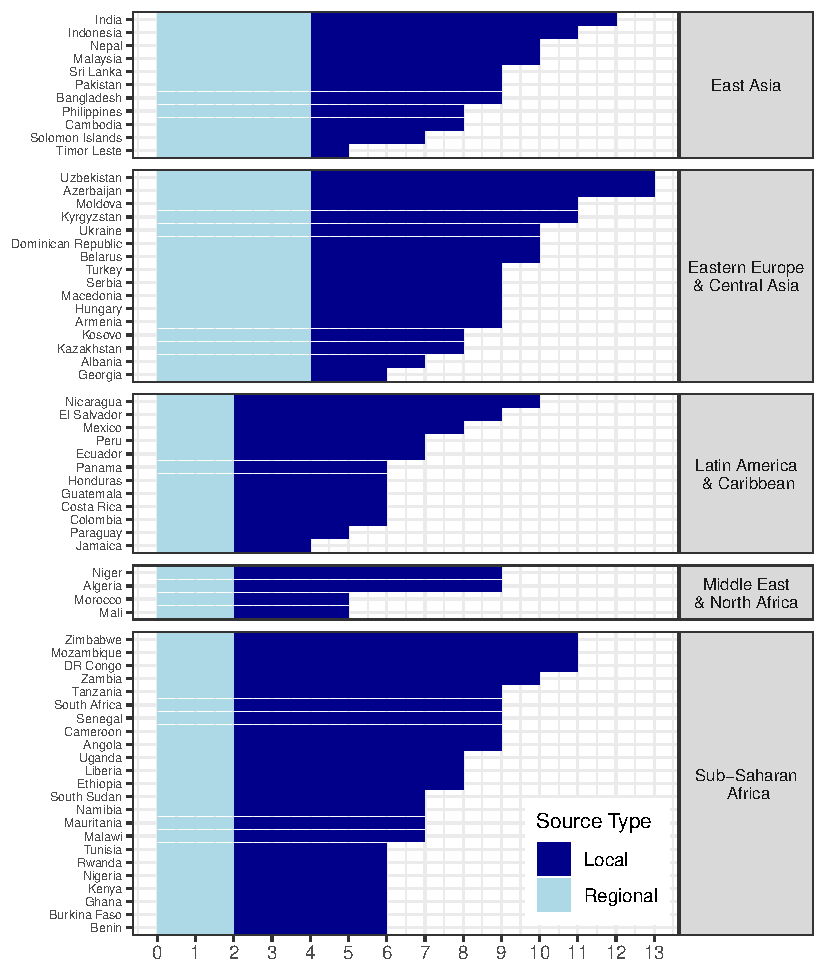
\includegraphics[keepaspectratio]{appendix_PoliticalAnalysis_Summer2026_files/figure-pdf/fig-source-distribution-1.pdf}}

}

\caption{\label{fig-source-distribution}Number of domestic and regional
media outlets in the HQMARC corpus by country}

\end{figure}%

\begin{figure}[H]

\centering{

\pandocbounded{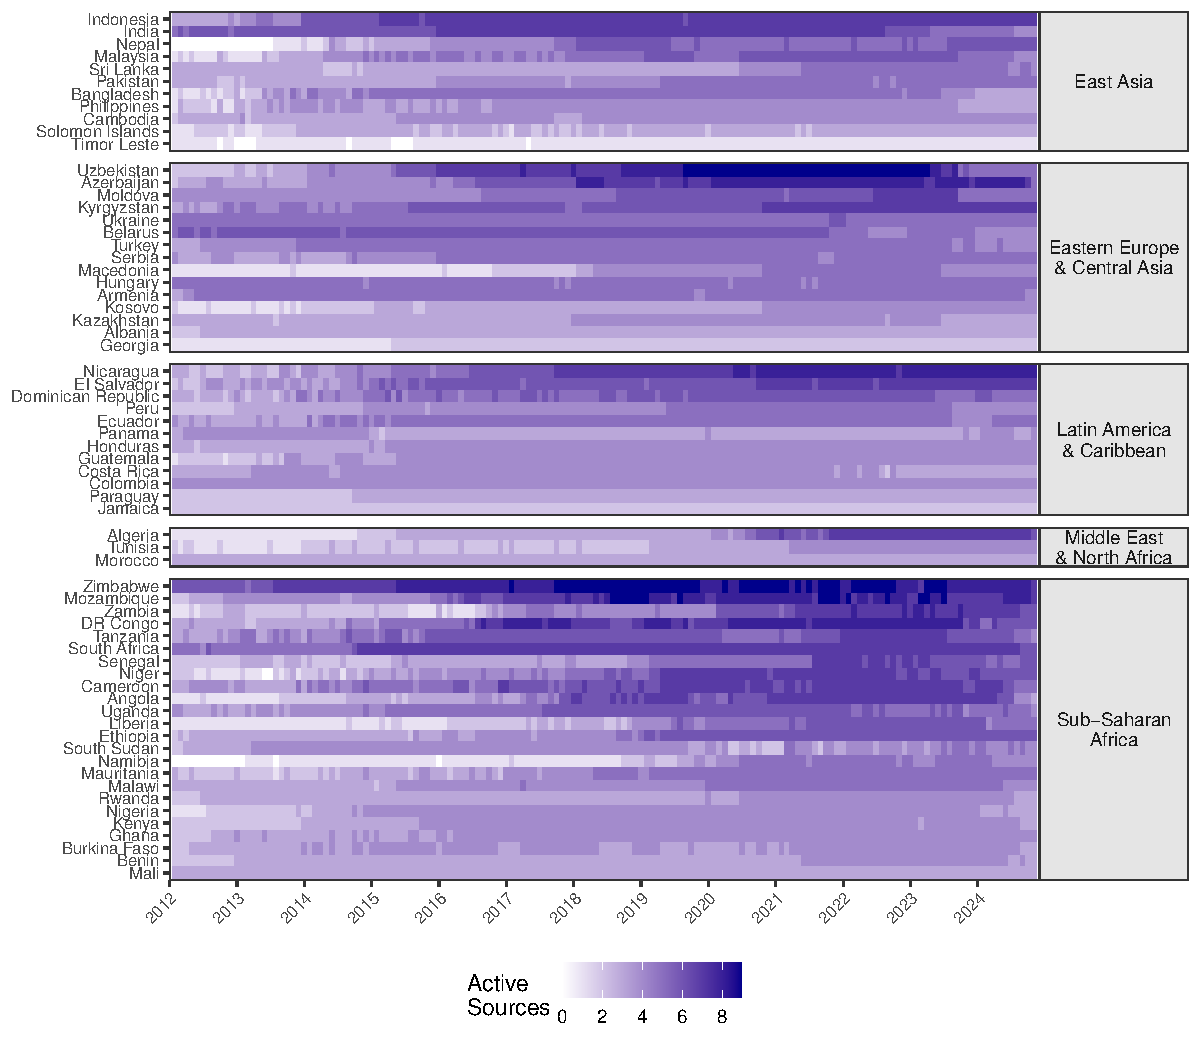
\includegraphics[keepaspectratio]{appendix_PoliticalAnalysis_Summer2026_files/figure-pdf/fig-source-active-1.pdf}}

}

\caption{\label{fig-source-active}Number of Active Domestic Sources by
Country-Month}

\end{figure}%

\subsection{Section 2: Languages in
HQMARC}\label{section-2-languages-in-hqmarc}

The \emph{HQMARC} corpus includes domestic media outlets publishing in
36 languages. These languages include Afrikaans, Albanian, Amharic,
Arabic, Armenian, Azerbaijani, Belarusian, Bengali, Chinese, English,
French, Georgian, Hindi, Hungarian, Indonesian, Kazakh, Central Khmer,
Kinyarwanda, Kongo, Macedonian, Malay, Nepali, Portuguese, Romanian,
Russian, Sinhala, Spanish, Serbian, Swahili, Tagalog, Turkish,
Ukrainian, Urdu, Uzbek, Zulu. Below, we provide the languages associated
with media outlets in each country using the language ISO codes.

\begin{table}[!h]
\centering
\caption{Eastern Europe \& Central Asia}
\centering
\fontsize{10}{12}\selectfont
\begin{tabular}[t]{l|l}
\hline
Country & Languages\\
\hline
Albania & sq, en\\
Armenia & hy, ru\\
Azerbaijan & en, az, ru\\
Belarus & be, ru\\
Georgia & ka, en\\
Hungary & hu\\
Kazakhstan & kk, ru, en\\
Kosovo & sq\\
Kyrgyzstan & en, ru, kg\\
Macedonia & sq, en, mk\\
Moldova & ro, ru, en\\
Serbia & sr\\
Turkey & tr\\
Ukraine & uk, ru, en\\
Uzbekistan & en, ru, uz\\
\hline
\end{tabular}
\end{table}

\begin{table}[!h]
\centering
\caption{Middle East \& North Africa}
\centering
\fontsize{10}{12}\selectfont
\begin{tabular}[t]{l|l}
\hline
Country & Languages\\
\hline
Algeria & fr, ar\\
Morocco & ar, fr\\
Tunisia & fr, ar\\
\hline
\end{tabular}
\end{table}

\begin{table}[!h]
\centering
\caption{Latin America \& Caribbean}
\centering
\fontsize{10}{12}\selectfont
\begin{tabular}[t]{l|l}
\hline
Country & Languages\\
\hline
Colombia & es\\
Costa Rica & es, en\\
Dominican Republic & es\\
Ecuador & es\\
El Salvador & es, en\\
Guatemala & es\\
Honduras & es, en\\
Jamaica & en\\
Nicaragua & es\\
Panama & es\\
Paraguay & es\\
Peru & es\\
\hline
\end{tabular}
\end{table}

\begin{table}[!h]
\centering
\caption{East Asia}
\centering
\fontsize{10}{12}\selectfont
\begin{tabular}[t]{l|l}
\hline
Country & Languages\\
\hline
Bangladesh & bn\\
Cambodia & km, en\\
India & en, hi\\
Indonesia & en, id\\
Malaysia & en, ms, zh\\
Nepal & ne, en\\
Pakistan & ur, en\\
Philippines & en, tl\\
Solomon Islands & en\\
Sri Lanka & en, si\\
Timor Leste & tet, pt\\
\hline
\end{tabular}
\end{table}

\begin{table}[!h]
\centering
\caption{Sub-Saharan Africa}
\centering
\fontsize{10}{12}\selectfont
\begin{tabular}[t]{l|l}
\hline
Country & Languages\\
\hline
Angola & pt\\
Benin & fr\\
Burkina Faso & fr\\
Cameroon & fr\\
DR Congo & fr\\
Ethiopia & en, am\\
Ghana & en\\
Kenya & en\\
Liberia & en\\
Malawi & en\\
Mali & fr\\
Mauritania & fr, ar\\
Mozambique & pt, en\\
Namibia & en\\
Niger & fr\\
Nigeria & en\\
Rwanda & en, fr, rw\\
Senegal & fr\\
South Africa & af, en, zu\\
South Sudan & en, ar\\
Tanzania & en, sw\\
Uganda & en\\
Zambia & en\\
Zimbabwe & en\\
\hline
\end{tabular}
\end{table}

\clearpage

\subsection{Section 3: Digital News
Sources}\label{section-3-digital-news-sources}

In this section, we list the individual sources included in
\emph{HQMARC}. First, we list our international sources and regional
sources. Second, we list the sources associated with each country,
organized by region.

\subsubsection{International Sources}\label{international-sources}

\begin{itemize}
\tightlist
\item
  aljazeera.com
\item
  bbc.com
\item
  csmonitor.com
\item
  france24.com
\item
  nytimes.com
\item
  reuters.com
\item
  scmp.com
\item
  theguardian.com
\item
  themoscowtimes.com
\item
  washingtonpost.com
\item
  wsj.com
\item
  lemonde.fr
\item
  liberation.fr
\item
  elpais.com
\item
  lefigaro.fr
\end{itemize}

\subsubsection{Eastern Europe \& Central Asia Regional
Sources}\label{eastern-europe-central-asia-regional-sources}

\begin{itemize}
\tightlist
\item
  balkaninsight.com
\item
  euronews.com
\item
  iwpr.net
\item
  neweasterneurope.eu
\end{itemize}

\subsubsection{Middle East \& North Africa Regional
Sources}\label{middle-east-north-africa-regional-sources}

\begin{itemize}
\tightlist
\item
  africanews.com
\item
  theeastafrican.co.ke
\end{itemize}

\subsubsection{Latin America \& Caribbean Regional
Sources}\label{latin-america-caribbean-regional-sources}

\begin{itemize}
\tightlist
\item
  cnnespanol.cnn.com
\item
  telemundo.com
\end{itemize}

\subsubsection{East Asia Regional
Sources}\label{east-asia-regional-sources}

\begin{itemize}
\tightlist
\item
  asia.nikkei.com
\item
  asiatimes.com
\item
  indiatimes.com
\item
  timesofindia.indiatimes.com
\end{itemize}

\subsubsection{Sub-Saharan Africa Regional
Sources}\label{sub-saharan-africa-regional-sources}

\begin{itemize}
\tightlist
\item
  africanews.com
\item
  theeastafrican.co.ke
\end{itemize}

\subsubsection{Eastern Europe \& Central Asia Local
Sources}\label{eastern-europe-central-asia-local-sources}

Albania :

\begin{itemize}
\tightlist
\item
  gazetatema.net
\item
  panorama.com.al
\item
  telegraf.al
\end{itemize}

Armenia :

\begin{itemize}
\tightlist
\item
  azatutyun.am
\item
  aravot.am
\item
  168.am
\item
  1in.am
\item
  golosarmenii.am
\end{itemize}

Azerbaijan :

\begin{itemize}
\tightlist
\item
  azeritimes.com
\item
  azadliq.info
\item
  abzas.org
\item
  turan.az
\item
  zerkalo.az
\item
  mikroskopmedia.com
\item
  xalqcebhesi.az
\item
  musavat.com
\item
  ru.echo.az
\end{itemize}

Belarus :

\begin{itemize}
\tightlist
\item
  nashaniva.by
\item
  novychas.by
\item
  nv-online.info
\item
  belgazeta.by
\item
  zviazda.by
\item
  sb.by
\end{itemize}

Georgia :

\begin{itemize}
\tightlist
\item
  ambebi.ge
\item
  georgiatoday.ge
\end{itemize}

Hungary :

\begin{itemize}
\tightlist
\item
  index.hu
\item
  24.hu
\item
  168.hu
\item
  hvg.hu
\item
  demokrata.hu
\end{itemize}

Kazakhstan :

\begin{itemize}
\tightlist
\item
  caravan.kz
\item
  diapazon.kz
\item
  kaztag.kz
\item
  rus.azattyq.org
\end{itemize}

Kosovo :

\begin{itemize}
\tightlist
\item
  kosova-sot.info
\item
  balkaninsight.com
\item
  prishtinainsight.com
\item
  botasot.info
\end{itemize}

Kyrgyzstan :

\begin{itemize}
\tightlist
\item
  akipress.com
\item
  24.kg
\item
  kloop.kg
\item
  super.kg
\item
  vb.kg
\item
  kaktus.kg
\item
  kaktus.media
\end{itemize}

Macedonia :

\begin{itemize}
\tightlist
\item
  koha.mk
\item
  slobodenpecat.mk
\item
  makfax.com.mk
\item
  skopjediem.com
\item
  novamakedonija.com.mk
\end{itemize}

Moldova :

\begin{itemize}
\tightlist
\item
  timpul.md
\item
  tribuna.md
\item
  unimedia.info
\item
  voceabasarabiei.md
\item
  publika.md
\item
  ipn.md
\item
  zdg.md
\end{itemize}

Serbia :

\begin{itemize}
\tightlist
\item
  rs.n1info.com
\item
  juznevesti.com
\item
  insajder.net
\item
  danas.rs
\item
  balkaninsight.com
\end{itemize}

Turkey :

\begin{itemize}
\tightlist
\item
  diken.com.tr
\item
  t24.com.tr
\item
  sozcu.com.tr
\item
  posta.com.tr
\item
  sabah.com.tr
\end{itemize}

Ukraine :

\begin{itemize}
\tightlist
\item
  delo.ua
\item
  interfax.com.ua
\item
  kp.ua
\item
  pravda.com.ua
\item
  kyivpost.com
\item
  kyivindependent.com
\end{itemize}

Uzbekistan :

\begin{itemize}
\tightlist
\item
  fergana.ru
\item
  kun.uz
\item
  gazeta.uz
\item
  podrobno.uz
\item
  batafsil.uz
\item
  sof.uz
\item
  anhor.uz
\item
  asiaterra.info
\item
  daryo.uz
\end{itemize}

\subsubsection{Middle East \& North Africa Local
Sources}\label{middle-east-north-africa-local-sources}

Algeria :

\begin{itemize}
\tightlist
\item
  twala.info
\item
  24hdz.com
\item
  echoroukonline.com
\item
  elkhabar.com
\item
  el-massa.com
\item
  elwatan-dz.com
\item
  echaab.dz
\end{itemize}

Morocco :

\begin{itemize}
\tightlist
\item
  leconomiste.com
\item
  lematin.ma
\item
  assabah.ma
\end{itemize}

Tunisia :

\begin{itemize}
\tightlist
\item
  assarih.com
\item
  babnet.net
\item
  jomhouria.com
\item
  lapresse.tn
\end{itemize}

\subsubsection{Latin America \& Caribbean Local
Sources}\label{latin-america-caribbean-local-sources}

Colombia :

\begin{itemize}
\tightlist
\item
  elcolombiano.com
\item
  elespectador.com
\item
  elheraldo.co
\item
  eltiempo.com
\end{itemize}

Costa Rica :

\begin{itemize}
\tightlist
\item
  larepublica.net
\item
  news.co.cr
\item
  ticotimes.net
\item
  diarioextra.com
\end{itemize}

Dominican Republic :

\begin{itemize}
\tightlist
\item
  diariolibre.com
\item
  listindiario.com
\item
  elnacional.com.do
\item
  hoy.com.do
\item
  elcaribe.com.do
\item
  elviajero.com.do
\end{itemize}

Ecuador :

\begin{itemize}
\tightlist
\item
  elcomercio.com
\item
  eldiario.ec
\item
  elnorte.ec
\item
  eluniverso.com
\item
  metroecuador.com.ec
\end{itemize}

El Salvador :

\begin{itemize}
\tightlist
\item
  laprensagrafica.com
\item
  elfaro.net
\item
  elsalvador.com
\item
  diario.elmundo.sv
\item
  diarioelsalvador.com
\item
  revistafactum.com
\item
  gatoencerrado.news
\end{itemize}

Guatemala :

\begin{itemize}
\tightlist
\item
  prensalibre.com
\item
  republica.gt
\item
  lahora.gt
\item
  soy502.com
\end{itemize}

Honduras :

\begin{itemize}
\tightlist
\item
  elheraldo.hn
\item
  laprensa.hn
\item
  proceso.hn
\item
  tiempo.hn
\end{itemize}

Jamaica :

\begin{itemize}
\tightlist
\item
  jamaica-gleaner.com
\item
  jamaicaobserver.com
\end{itemize}

Nicaragua :

\begin{itemize}
\tightlist
\item
  confidencial.com.ni
\item
  laprensani.com
\item
  nuevaya.com.ni
\item
  articulo66.com
\item
  laverdadnica.com
\item
  ondalocalni.com
\item
  canal2tv.com
\item
  lajornadanet.com
\end{itemize}

Panama :

\begin{itemize}
\tightlist
\item
  elsiglo.com.pa
\item
  critica.com.pa
\item
  panamaamerica.com.pa
\item
  newsroompanama.com
\end{itemize}

Paraguay :

\begin{itemize}
\tightlist
\item
  abc.com.py
\item
  lanacion.com.py
\item
  ultimahora.com
\end{itemize}

Peru :

\begin{itemize}
\tightlist
\item
  elcomercio.pe
\item
  gestion.pe
\item
  larepublica.pe
\item
  ojo-publico.com
\item
  idl-reporteros.pe
\end{itemize}

\subsubsection{East Asia Local Sources}\label{east-asia-local-sources}

Bangladesh :

\begin{itemize}
\tightlist
\item
  prothomalo.com
\item
  bd-pratidin.com
\item
  kalerkantho.com
\item
  jugantor.com
\item
  dailyjanakantha.com
\end{itemize}

Cambodia :

\begin{itemize}
\tightlist
\item
  kohsantepheapdaily.com.kh
\item
  moneaksekar.com
\item
  phnompenhpost.com
\item
  cambodiadaily.com
\end{itemize}

India :

\begin{itemize}
\tightlist
\item
  amarujala.com
\item
  indianexpress.com
\item
  thehindu.com
\item
  hindustantimes.com
\item
  deccanherald.com
\item
  firstpost.com
\item
  indiatimes.com
\item
  timesofindia.indiatimes.com
\end{itemize}

Indonesia :

\begin{itemize}
\tightlist
\item
  thejakartapost.com
\item
  jawapos.com
\item
  kompas.com
\item
  mediaindonesia.com
\item
  sindonews.com
\item
  beritasatu.com
\item
  hariansib.com
\end{itemize}

Malaysia :

\begin{itemize}
\tightlist
\item
  malaymail.com
\item
  nst.com.my
\item
  thestar.com.my
\item
  utusan.com.my
\item
  thesun.my
\item
  malaysiakini.com
\end{itemize}

Nepal :

\begin{itemize}
\tightlist
\item
  onlinekhabar.com
\item
  english.onlinekhabar.com
\item
  en.setopati.com
\item
  thehimalayantimes.com
\item
  kathmandupost.com
\item
  nepalitimes.com
\end{itemize}

Pakistan :

\begin{itemize}
\tightlist
\item
  jang.com.pk
\item
  nation.com.pk
\item
  dailytimes.com.pk
\item
  pakobserver.net
\item
  tribune.com.pk
\end{itemize}

Philippines :

\begin{itemize}
\tightlist
\item
  mb.com.ph
\item
  manilastandard.net
\item
  inquirer.net
\item
  manilatimes.net
\end{itemize}

Solomon Islands :

\begin{itemize}
\tightlist
\item
  solomonstarnews.com
\item
  solomontimes.com
\item
  sibconline.com.sb
\end{itemize}

Sri Lanka :

\begin{itemize}
\tightlist
\item
  dailymirror.lk
\item
  island.lk
\item
  divaina.lk
\item
  adaderana.lk
\item
  lankadeepa.lk
\end{itemize}

Timor Leste :

\begin{itemize}
\tightlist
\item
  thediliweekly.com
\end{itemize}

\subsubsection{Sub-Saharan Africa Local
Sources}\label{sub-saharan-africa-local-sources}

Angola :

\begin{itemize}
\tightlist
\item
  opais.co.ao
\item
  jornalf8.net
\item
  angola24horas.com
\item
  portaldeangola.com
\item
  angola-online.net
\item
  vozdeangola.com
\item
  jornaldeangola.ao
\end{itemize}

Benin :

\begin{itemize}
\tightlist
\item
  lanouvelletribune.info
\item
  news.acotonou.com
\item
  lematinal.media
\item
  levenementprecis.com
\end{itemize}

Burkina Faso :

\begin{itemize}
\tightlist
\item
  lefaso.net
\item
  burkina24.com
\item
  evenement-bf.net
\item
  laborpresse.net
\end{itemize}

Cameroon :

\begin{itemize}
\tightlist
\item
  journalducameroun.com
\item
  camerounweb.com
\item
  237actu.com
\item
  237online.com
\item
  cameroonvoice.com
\item
  lebledparle.com
\item
  thesunnewspaper.cm
\end{itemize}

DR Congo :

\begin{itemize}
\tightlist
\item
  radiookapi.net
\item
  lesoftonline.net
\item
  acpcongo.com
\item
  lephareonline.net
\item
  groupelavenir.org
\item
  matininfos.net
\item
  cas-info.ca
\item
  actualite.cd
\item
  7sur7.cd
\end{itemize}

Ethiopia :

\begin{itemize}
\tightlist
\item
  addisfortune.news
\item
  addisstandard.com
\item
  capitalethiopia.com
\item
  thereporterethiopia.com
\item
  ethiopianmonitor.com
\item
  addisadmassnews.com
\end{itemize}

Ghana :

\begin{itemize}
\tightlist
\item
  dailyguidenetwork.com
\item
  ghanaweb.com
\item
  graphic.com.gh
\item
  newsghana.com.gh
\end{itemize}

Kenya :

\begin{itemize}
\tightlist
\item
  kbc.co.ke
\item
  citizen.digital
\item
  nation.africa
\item
  theeastafrican.co.ke
\end{itemize}

Liberia :

\begin{itemize}
\tightlist
\item
  thenewdawnliberia.com
\item
  liberianobserver.com
\item
  analystliberiaonline.com
\item
  frontpageafricaonline.com
\item
  inquirernewspaper.com
\item
  thenewsnewspaper.online
\end{itemize}

Malawi :

\begin{itemize}
\tightlist
\item
  mwnation.com
\item
  nyasatimes.com
\item
  times.mw
\item
  faceofmalawi.com
\item
  malawivoice.com
\end{itemize}

Mali :

\begin{itemize}
\tightlist
\item
  maliweb.net
\item
  malijet.com
\item
  news.abamako.com
\end{itemize}

Mauritania :

\begin{itemize}
\tightlist
\item
  alwiam.info
\item
  lecalame.info
\item
  journaltahalil.com
\item
  alakhbar.info
\item
  saharamedias.net
\end{itemize}

Mozambique :

\begin{itemize}
\tightlist
\item
  correiodabeiraserra.com
\item
  canal.co.mz
\item
  mmo.co.mz
\item
  cartamz.com
\item
  verdade.co.mz
\item
  clubofmozambique.com
\item
  portalmoznews.com
\item
  jornaldomingo.co.mz
\item
  tvm.co.mz
\end{itemize}

Namibia :

\begin{itemize}
\tightlist
\item
  namibian.com.na
\item
  confidentenamibia.com
\item
  thevillager.com.na
\item
  observer24.com.na
\item
  informante.web.na
\end{itemize}

Niger :

\begin{itemize}
\tightlist
\item
  actuniger.com
\item
  nigerinter.com
\item
  lesahel.org
\item
  tamtaminfo.com
\item
  airinfoagadez.com
\item
  nigerexpress.info
\item
  journalduniger.com
\end{itemize}

Nigeria :

\begin{itemize}
\tightlist
\item
  guardian.ng
\item
  thenewsnigeria.com.ng
\item
  vanguardngr.com
\item
  thenationonlineng.net
\end{itemize}

Rwanda :

\begin{itemize}
\tightlist
\item
  newtimes.co.rw
\item
  therwandan.com
\item
  kigalitoday.com
\item
  umuseke.rw
\end{itemize}

Senegal :

\begin{itemize}
\tightlist
\item
  xalimasn.com
\item
  lesoleil.sn
\item
  enqueteplus.com
\item
  lasnews.sn
\item
  ferloo.com
\item
  nouvelobs.com
\item
  sudquotidien.sn
\end{itemize}

South Africa :

\begin{itemize}
\tightlist
\item
  timeslive.co.za
\item
  news24.com
\item
  dailysun.co.za
\item
  sowetanlive.co.za
\item
  isolezwe.co.za
\item
  iol.co.za
\item
  son.co.za
\end{itemize}

South Sudan :

\begin{itemize}
\tightlist
\item
  radiotamazuj.org
\item
  sudantribune.com
\item
  paanluelwel.com
\item
  onecitizendaily.com
\item
  eyeradio.org
\end{itemize}

Tanzania :

\begin{itemize}
\tightlist
\item
  ippmedia.com
\item
  dailynews.co.tz
\item
  habarileo.co.tz
\item
  thecitizen.co.tz
\item
  mtanzania.co.tz
\item
  jamhurimedia.co.tz
\item
  mzalendo.co.tz
\end{itemize}

Uganda :

\begin{itemize}
\tightlist
\item
  monitor.co.ug
\item
  observer.ug
\item
  newvision.co.ug
\item
  nilepost.co.ug
\item
  sunrise.ug
\item
  eagle.co.ug
\end{itemize}

Zambia :

\begin{itemize}
\tightlist
\item
  lusakatimes.com
\item
  mwebantu.com
\item
  diggers.news
\item
  openzambia.com
\item
  lusakavoice.com
\item
  dailynationzambia.com
\item
  zambianewsnetwork.com
\item
  zambianobserver.com
\end{itemize}

Zimbabwe :

\begin{itemize}
\tightlist
\item
  thestandard.co.zw
\item
  theindependent.co.zw
\item
  herald.co.zw
\item
  chronicle.co.zw
\item
  newsday.co.zw
\item
  thezimbabwean.co
\item
  zimbabwesituation.com
\item
  newzimbabwevision.com
\item
  zimlive.com
\end{itemize}

\subsection{Section 4: Assessing Outlet
Independence}\label{section-4-assessing-outlet-independence}

To ensure data quality, \emph{HQMARC} aims to capture news from the most
trustworthy media outlets available for each country. During the
construction of \emph{HQMARC}, our team scraped each source every three
months to capture new articles published since the last scrape. For
countries ranked outside of the top 100 for media freedom by Reporters
Without Borders, we consider their media environments restrictive. For
all sources in countries with restrictive media environments, we
investigate potential sources of bias for all our sources at a
three-month frequency. These frequent bias checks are due to changes in
coverage of sources and changes in ownership of sources over times.

For countries with restrictive media environments, we aim to source at
least half of the articles from sources that are coded politically
independent. For countries where less than half of the articles are
collected from independent sources, we encourage users to apply
weighting.

Human coders follow detailed coding instructions to assess each outlet
according to Ideology (5-point scale from Right to Left), Independence
from the regime or opposition (Pro-regime, Opposition, or Independent),
and Ownership (Government owned or non-government owned). Coders begin
by consulting a list of public resources and performing a subjective
review of a sample of published articles. Coding instructions and
source-level bias data are available on our github at
\href{https://github.com/ML4PDevLab/MLP-data-intro/tree/main/source_metadata}{MLP-data-intro/source\_metadata/}.

\subsection{Section 5: Assessing and Comparing
Coverage}\label{section-5-assessing-and-comparing-coverage}

To demonstrate the importance of our custom workflow, we present a case
study comparing \emph{HQMARC's} coverage with that of several ``big
data'' media corpora, demonstrating that \emph{HQMARC} captures a
significantly more articles from high-quality domestic outlets. We then
demonstrate the pitfalls of relying on automated parsing tools without
human oversight.

We compare \emph{HQMARC's} coverage of three prominent Bangladeshi news
outlets to that of GDELT and Internet Archive. We focus on for
Bangladesh three reasons. First, Bangladeshi outlets publish a high
volume of articles relative to other countries, making them more likely
to attract automated crawlers. Second, the website architecture for each
outlet is straightforward, maximizing the likelihood that crawlers and
automated parsers will accurately retrieve articles. Third, many
Bangladeshi sources publish primarily in English, reducing the
additional hurdles of multilingual parsing. As a result, we regard these
outlets as a ``best-case scenario'' for large-scale media repositories.

Despite favorable conditions, we find notable differences between
\emph{HQMARC} and the aggregators. \emph{HQMARC's} coverage begins in
2013 for one source and in 2015 for the other two. However, GDELT does
not have any articles published before 2019 for any of the three
sources. Even after 2019, GDELT captures many fewer articles than
\emph{HQMARC}. For the source with the smallest disparity between
\emph{HQMARC} and GDELT, GDELT retrieves an average of 2,100 articles
per month, compared to 2,500 in \emph{HQMARC}. GDELT also includes
numerous broken links, redirects, duplicate articles, etc. that
\emph{HQMARC's} human review removed. In addition, GDELT's five-second
delay per query makes it extremely time-consuming to scrape a full
historical archive of this size. Across these three sources, Internet
Archive achieved coverage similar to that of \emph{HQMARC}, but more
than half of these urls were broken and no longer pointed to the a
webpage that contained the article text. Furthermore, collecting URLs
from Internet Archive for 2019--2023 required roughly two weeks from a
single source and returned many irrelevant and duplicate links not
contained in \emph{HQMARC}.

\section{Appendix B: Civic Space Definitions, Keywords, and Classifier
Performance}\label{appendix-b-civic-space-definitions-keywords-and-classifier-performance}

\subsection{Section 1: Event
Definitions}\label{section-1-event-definitions}

\begin{itemize}
\item
  Activism

  \begin{itemize}
  \tightlist
  \item
    Any activity by individuals, community organizations, or NGOs that
    involve some amount of lobbying, raising awareness, or collective
    action beyond just the donation of money. Importantly, this does not
    include protests or activities related to election campaigns.
  \item
    \textbf{Example:} ``Retired soldiers make up subsidiary of Just
    Cause.A group of retired soldiers met yesterday morning in a
    restaurant in the city of San Miguel to learn about the work of the
    Association Causa Justa, in order to organize a branch in the
    eastern part of the country.Jaime García, vice president of Causa
    Justa, explained that this association has been working for a couple
    of years to defend the interests of retired soldiers, and since then
    they have organized a branch in San Ana and now they intend to have
    another group.''
  \end{itemize}
\item
  Arrests

  \begin{itemize}
  \tightlist
  \item
    An institution within the government-controlled security apparatus
    --i.e.~the police, the military, or other-- apprehends people or
    groups of people who are part of an opposition movement or party, a
    civil society organization, a media organization, or a protest.
  \item
    \textbf{Example:} ``The Police in Abia on Wednesday arrested 51
    persons suspected to be members of the proscribed Indigenous People
    of Biafra, claiming they `operate as members of Judaism,' in
    Umuahia.''
  \end{itemize}
\item
  Censor

  \begin{itemize}
  \tightlist
  \item
    The government actively prevents free speech by individuals in the
    media, in public or online. This includes banning certain content
    from individual speech or news stories, dictating how certain
    concepts or people can be referred to in public speech, or directly
    dictating agenda setting for media organizations. This category also
    includes the government censoring internet websites, internet
    shutdowns, fines on independent media, limitations on foreign
    ownership of media outlets, and political actors gaining influence
    within media organizations. Magnitude is a scale (see below; try to
    determine the importance of the target with information given).
  \item
    \textbf{Example:} ``The Tanzanian government has suspended newspaper
    The Citizen for seven days after the publication ran a story on the
    falling value of the Tanzanian shilling.''
  \end{itemize}
\item
  Corruption

  \begin{itemize}
  \tightlist
  \item
    The abuse of entrusted power for private gain. This includes
    street-level corruption (for instance, bribes to police), high-level
    corruption (in public contracting, for instance), and legal actions
    around corruptions.
  \item
    \textbf{Example:} ``Ex-President Sarkozy gets Jail Sentence for
    Corruption in France''
  \end{itemize}
\item
  Coup

  \begin{itemize}
  \tightlist
  \item
    Changes in government or persistence of government that are not in
    the rules of succession or transition. Coups, refusing to cede
    power, or a power grab after an unfair election are examples of this
    event type. Peaceful government transitions are nonviolent transfers
    of power or legitimate continuity of government elected by
    democratic means and accepted by a majority of political forces.
    Code peaceful change as `1' in the direction column. Speech is the
    pledge to accept the result of an election (a threat of a coup falls
    under `political threat').
  \item
    \textbf{Example:} ``Forces loyal to Turkey's president quashed a
    coup attempt in a night of explosions, air battles and gunfire that
    left at least 161 people dead and 1,440 wounded, yesterday.
    President Recep Tayyip Erdogan vowed that those responsible ``will
    pay a heavy price for their treason''.
  \end{itemize}
\item
  Defamation Case

  \begin{itemize}
  \tightlist
  \item
    Cases in which an individual or a group related to an opposition
    movement or party, current or former government officials, a civil
    society organization, a media organization, a business leader, a
    member of a minority group, or a protest are accused, usually by a
    government official, of: directly defaming/libeling/slandering the
    government or one or some of its members. Alternatively, these are:
    strategic lawsuits against civic actors to intimidate public
    participation. This category is a subset of the `Legal Action' event
    type (see below).
  \item
    \textbf{Example:} ``A Phnom Penh court on Friday found veteran
    opposition chief Sam Rainsy guilty of defaming Prime Minister Hun
    Sen and ordered him to pay damages of \$1 million, the latest blow
    to an opposition crippled by legal cases this year.''
  \end{itemize}
\item
  Disaster

  \begin{itemize}
  \tightlist
  \item
    This category includes: (1) natural disasters such as earthquakes,
    hurricanes, floods, famines or food crises or any catastrophic event
    that results or may result in serious damage. loss of life, and/or
    political implications; (2) infrastructural accidents that can
    endanger the population --a dam or pipe bursting, the sinking of a
    ferry, etc.) The goal is to focus on the types of events that might
    reflect on government accountability and civic space, not minor
    events like traffic accidents. Note: this includes deaths or
    economic strife caused by disasters, including reports on
    deaths/infections caused by COVID-19.
  \item
    \textbf{Example:} ROMBO district residents in Kilimanjaro region are
    in danger of facing food shortage if concerted efforts to control
    wildlife in consuming crops are not employed.
  \end{itemize}
\item
  Election Activity

  \begin{itemize}
  \tightlist
  \item
    Reporting on regular electoral activities including the introduction
    of candidacies, the conduct of campaigns, the announcement of
    results, and the formal transfer of power for public office. This
    includes situations where the incumbent party/candidate retains
    power. Normal election results are an example of this event type.
    Specifically, this includes peaceful government transitions that are
    nonviolent transfers of power or legitimate continuity of government
    but does not include coups, which are accounted for separately.
  \item
    \textbf{Example:} ``The President of the Executive Board of the
    Serbian Progressive Party, Darko Glisic, said that the SNS won a
    convincing victory with 60.2 percent of the votes, based on the
    processed 221 out of 231 polling stations where the voting for the
    parliamentary elections in Serbia was repeated.''
  \end{itemize}
\item
  Election Irregularities

  \begin{itemize}
  \tightlist
  \item
    The altering or attempted altering through legal or extra-legal
    manipulation of the conduct, rules or results of elections or
    electoral processes. This could include
    rescheduling/postponing/cancelling regularly-scheduled elections,
    calling irregular elections or constitutional referenda, hampering
    the work of independent election observers, eroding the
    autonomy/authority of the electoral commission, as well as any other
    institutional change that directly affects the electoral process.
    This additionally could include the cancellation of party lists and
    the boycott of elections by opposition, as well as calls for
    recounts or other forms of contesting elections. Finally, this
    includes vote-buying, intimidation, or vote-rigging. This does not
    include standard election proceedings.
  \item
    \textbf{Example:} ``Nigeria's electoral authority has delayed
    presidential and national assembly elections by one week amidst
    protests from the two main opposition parties. The government
    alleged logistical problems with ballot delivery to justify the
    delay.''
  \end{itemize}
\item
  Legal Action

  \begin{itemize}
  \tightlist
  \item
    Legal action refers to the prosecution or investigation of criminal
    activity or disputes over government authority, as well as the
    trials, convictions or dismissals that result. This event is related
    to civic space if the targeted people are part of an opposition
    movement or party, current and former government officials, a civil
    society organization, an NGO, a media organization or member, a
    (legal or illegal) business leader, member of minority group, or a
    protest. This specifically does not include arrests, which are
    defined as its own event type. Defamation cases are a subset of
    `Legal Action' (see above).
  \item
    \textbf{Example:} ``Kosovo President is Indicted for War Crimes for
    Role in War with Serbia.''
  \end{itemize}
\item
  Legal Change

  \begin{itemize}
  \tightlist
  \item
    Legal change refers to any changes or proposed changes in the laws
    of a nation in such a way as to affect civic space. This includes
    legal restrictions on speech, political groups, NGOs, and the
    changing of constitutions as well as changing of the powers of the
    government. This also includes some restrictions on assembly, but
    does not include curfews and other martial law declarations, which
    are specifically covered by other event categories.
  \item
    \textbf{Example:} ``Venezuela's constituent assembly yesterday
    unanimously passed a law that mandates punishment including a prison
    sentence of up to 20 years for anyone who instigates hate or
    violence on the radio, television or via social media.''
  \end{itemize}
\item
  Cooperation

  \begin{itemize}
  \tightlist
  \item
    Domestic political, social, or business actors collaborate on one or
    a range of issues or demonstrate an intent to do so. This does not
    include intragovernmental cooperation, except for local and federal
    cooperation. Cooperation indicates a willingness for domestic actors
    to work together to resolve important issues. Cooperation involving
    international actors is not a civic space event, but is an RAI
    event.
  \item
    \textbf{Example:}
  \end{itemize}
\item
  Lethal Violence

  \begin{itemize}
  \tightlist
  \item
    Any action of aggression by a government entity, organized group or
    individual that results in the death of one or more people,
    excluding crimes of passion.
  \item
    \textbf{Example:} ``The Kaduna state government, Friday evening,
    disclosed that 33 women and children were killed by rebels in Kajuru
    local government of Kaduna state, less than twenty-four hours to the
    conduct of the presidential and parliamentary elections.''
  \end{itemize}
\item
  Martial Law

  \begin{itemize}
  \tightlist
  \item
    The executive branch declares a state of emergency or suspends,
    temporarily or indefinitely, the ability of citizens to gather or
    protest against the order.
  \item
    \textbf{Example:} ``On Wednesday, President Duterte approved the
    extension of martial law in the country's volatile south by a year
    due to continuing threats by Islamic State group-linked militants
    and communist insurgents.''
  \end{itemize}
\item
  Mobilize Security Forces

  \begin{itemize}
  \tightlist
  \item
    An event in which the government mobilizes police forces, military
    troops or government-affiliated militias.
  \item
    \textbf{Example:} ``More than 500 security personnel have being
    mobilised for Saturday's governorship election in Sokoto State, says
    the state commissioner of police (CP), Alhaji Adisa Bolanta.''
  \end{itemize}
\item
  Non-Lethal Violence

  \begin{itemize}
  \tightlist
  \item
    Any action of aggression by a government entity, organized group or
    individual that physically harms one or more people or property but
    does NOT result in death, excluding crimes of passion.
  \item
    \textbf{Example:} ``At least four persons were injured at Oruk Anam
    Local Government Area of Akwa Ibom State on during yesterday's
    national election. Reports claim that unknown assailants attempted
    to snatch ballot boxes while voting was still ongoing.''
  \end{itemize}
\item
  Protest

  \begin{itemize}
  \tightlist
  \item
    Planned or spontaneous public mobilization of a large group of
    people. Labor strikes, political rallies and riots are also included
    in this category. When protest events involve deaths, they are coded
    as lethal violence, but this does not apply for non-lethal violence
    incidents.
  \item
    \textbf{Example:} ``A reported two thousand people took to the
    streets yesterday in Nairobi to protest rising fuel prices, which
    have doubled since the beginning of the year.''
  \end{itemize}
\item
  Purge/Replace

  \begin{itemize}
  \tightlist
  \item
    Purge/replace refers to the removal, firing or resignation of
    individuals from a government position or the replacement of
    previously removed individuals, including when the removals/firings
    themselves are not directly mentioned in the article. This includes
    the resignation of the chief executive. This description applies to
    purging of targets such as the bureaucracy, courts, military,
    police, state-owned companies, or members of political parties,
    among others.
  \item
    \textbf{Example:} ``Poland's government carried out a sweeping purge
    of the Supreme Court on Tuesday night, eroding the judiciary's
    independence, escalating a confrontation with the European Union
    over the rule of law and further dividing this nation.''
  \end{itemize}
\item
  Raid

  \begin{itemize}
  \tightlist
  \item
    Individuals or organizations are assaulted or aggressively coerced.
    Their property may be encroached or damaged as a result. Examples
    include a raid on newspaper offices. Victims themselves suffer no
    physical harm. This category also includes the government shutting
    down opposition organizations, NGOs, etc.
  \item
    \textbf{Example:} ``A Vanguard newspaper office located on Bassey
    Duke Street was, yesterday afternoon, raided by hoodlums, who carted
    away large sums of money and destroyed computers and other
    equipment.''
  \end{itemize}
\item
  Threats

  \begin{itemize}
  \tightlist
  \item
    A statement of a clear and explicit intention to inflict pain,
    injury, damage, or other hostile action on an individual or
    organization. Our targets and actors of interest are part of an
    opposition movement, the media, a political party, government, or a
    civil society organization.
  \item
    \textbf{Example 1:} ``A top Kenyan newspaper published a fake death
    notice of a prominent opposition financier on Wednesday, a bizarre
    error that rights groups interpreted as another sign of an
    anti-democratic slide. The Daily Nation apologized by mid-morning
    for publishing the funeral announcement for businessman Jimi
    Wanjigi, whose picture, history and family details were used but
    whose name was slightly altered. The paper said the ad was published
    in error and it was working with police to uncover who placed it.
    After a week of arrests of opposition politicians and a crackdown on
    independent media, a prominent rights campaigner said the
    announcement amounted to a death threat to Wanjigi, who funded
    opposition leader Raila Odinga's election campaign last year and
    whose house was raided by police in October.''
  \item
    \textbf{Example 2:} ``Nigeria's main labor unions threatened a
    nationwide strike over recent increases in gas prices.''
  \end{itemize}
\end{itemize}

\subsection{Section 2 Keywords and Their
Use}\label{section-2-keywords-and-their-use}

This document lists the categories where keywords are currently being
deployed as well as a brief explanation for their use.

\textbf{Legal Action}

\begin{itemize}
\tightlist
\item
  Keyword lists

  \begin{itemize}
  \tightlist
  \item
    Keyword list one: case \textbar{} lawsuit \textbar sue \textbar{}
    suit \textbar{} trial \textbar{} court \textbar{} charge \textbar{}
    rule \textbar{} sentence \textbar{} judge
  \item
    Keyword list two: defamation \textbar{} defame \textbar libel
    \textbar{} slander \textbar{} insult \textbar{} disparage \textbar{}
    lese majeste \textbar{} lese-majeste \textbar{} lese majesty
    \textbar{} reputation
  \end{itemize}
\item
  Purpose of Keywords

  \begin{itemize}
  \tightlist
  \item
    The purpose of these keywords is to move articles from legal action
    that are actually defamation case to the appropriate category. There
    is no longer a defamation case category, it is now entirely a subset
    of legal action. The first set of keywords filter out any instances
    where there are accusations of defamation/libel/slander that are not
    actual cases, but merely statements. The second set of keywords
    ensures that the cases are actually related to defamation, since we
    found that oftentimes, non-defamation cases where being assigned to
    this event category. The process is two-fold, requiring a key word
    from both lists.
  \item
    If keyword from both lists are not present, the article is left as
    legal action
  \end{itemize}
\end{itemize}

\textbf{Censor}

\begin{itemize}
\tightlist
\item
  Keyword list: Freedom \textbar{} assembly \textbar{} association
  \textbar{} movement \textbar{} independent \textbar{} independence
  \textbar{} succession \textbar{} demonstrate \textbar{} demonstration
  \textbar{} repression \textbar{} repressive \textbar{} crackdown
  \textbar{} draconian \textbar{} intimidate \textbar{} censoring
  \textbar{} controversial \textbar{} censor \textbar{} muzzle
  \textbar{} restrictive \textbar{} restrict \textbar{} authoritarian
  \textbar{} non-governmental organizations \textbar{} NGOs \textbar{}
  media \textbar{} parties \textbar{} civil society \textbar{}
  opposition \textbar{} critics \textbar{} opponents \textbar{} human
  rights groups \textbar{} arbitrary \textbar{} stifling \textbar{} ban
  \textbar{} strict \textbar{} boycott \textbar{} protests \textbar{}
  dissent \textbar{} demonstrators \textbar{} journal.* \textbar{}
  newspaper \textbar{} media \textbar{} outlet \textbar{} censor
  \textbar{} reporter \textbar{} broadcast.* \textbar{} correspondent
  \textbar{} press \textbar{} magazine \textbar{} paper \textbar{} black
  out \textbar{} blacklist \textbar{} suppress \textbar{} speaking
  \textbar{} false news \textbar{} fake news \textbar{} radio \textbar{}
  commentator \textbar{} blogger \textbar{} opposition voice \textbar{}
  voice of the opposition \textbar{} speech \textbar{} broadcast
  \textbar{} publish \textbar{} limit.* \textbar{} independ.* \textbar{}
  repress.* \textbar{} journalist \textbar{} newspaper \textbar{}
  reporter \textbar{} internet \textbar{} telecommunications \textbar{}
  magazine \textbar{} shut down \textbar{} broadcast \textbar{} radio
\item
  Purpose of Keywords

  \begin{itemize}
  \tightlist
  \item
    The purpose of these keywords is to filter out instances where
    restrictions are applied that are not censorship. This was created
    primarily in response to closings of schools, businesses, and
    government offices in relation to COVID-19, which were frequently
    classified as censorship.
  \item
    If one of the keywords is not present in the article, it is
    reclassified as -999
  \end{itemize}
\end{itemize}

\textbf{Legal Action/Purge/Arrest}

\begin{itemize}
\tightlist
\item
  Keyword list

  \begin{itemize}
  \tightlist
  \item
    embezzle \textbar{} embezzled \textbar{} embezzling \textbar{}
    embezzlement \textbar{} bribe \textbar{} bribes \textbar{} bribed
    \textbar{} bribing \textbar{} gift \textbar{} gifts \textbar{}
    gifted \textbar{} fraud \textbar{} fraudulent \textbar{} corrupt
    \textbar{} corruption \textbar{} procure \textbar{} procured
    \textbar{} procurement \textbar{} budget \textbar{} assets
    \textbar{} irregularities \textbar{} graft \textbar{} enrich
    \textbar{} enriched \textbar{} enrichment \textbar{} laundering
    \textbar{} fraudulent.
  \end{itemize}
\item
  Purpose of Keywords

  \begin{itemize}
  \tightlist
  \item
    The purpose of these keywords is to assign a second event category
    to those articles in arrest, purge, and legal action that also
    feature corruption. Articles in those categories that feature these
    words are double counted as both corruption and the original
    category.
  \end{itemize}
\end{itemize}

\textbf{Corruption}

\begin{itemize}
\tightlist
\item
  Keyword lists

  \begin{itemize}
  \tightlist
  \item
    For arrest: arrest; detain; apprehend; capture; custody; imprison;
    jail
  \item
    For legal action: legal process; case\emph{; investigate}; appeal;
    charged; prosecute*; case; lawsuit; sue; suit; trial; court; charge;
    rule; sentence; judge
  \item
    For purge: resign\emph{; fire}; dismiss; sack; replace; quit.
  \end{itemize}
\item
  Purpose of Keywords

  \begin{itemize}
  \tightlist
  \item
    The purpose of these keywords is to assign a second event category
    to those articles in corruption that also feature arrests, legal
    action, and purges. Articles in those categories that feature these
    words are double counted as both corruption and the original
    category.
  \end{itemize}
\end{itemize}

\#\#Section 3: Classifier Performance

\begin{longtable}[]{@{}llll@{}}
\caption{Performance metrics for fine-tuned RoBERTa classification
model. -999}\label{tbl-roberta}\tabularnewline
\toprule\noalign{}
Event Category & Precision & Recall & F1 \\
\midrule\noalign{}
\endfirsthead
\toprule\noalign{}
Event Category & Precision & Recall & F1 \\
\midrule\noalign{}
\endhead
\bottomrule\noalign{}
\endlastfoot
\textbf{Arrest} & 0.91 & 0.88 & 0.89 \\
\textbf{Protest} & 0.85 & 0.98 & 0.91 \\
\textbf{Legal action} & 0.77 & 0.75 & 0.76 \\
\textbf{Disaster} & 0.87 & 0.86 & 0.86 \\
\textbf{Censor} & 0.76 & 0.95 & 0.84 \\
\textbf{Election activity} & 0.78 & 0.84 & 0.81 \\
\textbf{Election irregularities} & 0.72 & 0.68 & 0.70 \\
\textbf{Activism} & 0.95 & 0.83 & 0.88 \\
\textbf{State of Emergency} & 0.92 & 0.90 & 0.91 \\
\textbf{Coup} & 0.68 & 0.83 & 0.75 \\
\textbf{Non-lethal violence} & 0.79 & 0.81 & 0.80 \\
\textbf{Lethal violence} & 0.90 & 0.82 & 0.86 \\
\textbf{Corruption} & 0.74 & 0.71 & 0.73 \\
\textbf{Legal change} & 0.84 & 0.80 & 0.82 \\
\textbf{Security mobilization} & 0.83 & 0.77 & 0.80 \\
\textbf{Purge} & 0.91 & 0.86 & 0.88 \\
\textbf{Threats} & 1.00 & 0.78 & 0.88 \\
\textbf{Raid} & 1.00 & 0.83 & 0.91 \\
\textbf{Irrelevant events} & 0.81 & 0.79 & 0.80 \\
\end{longtable}

\section{Appendix C: Descriptive
Maps}\label{appendix-c-descriptive-maps}

These temporal world maps provide a comprehensive overview of civic
space coverage patterns across all 65 developing countries in the HQMARC
corpus from 2012 to 2024. The maps reveal significant variation in both
the intensity of civic space reporting and the types of events that
dominate coverage across countries and over time. Geographic clustering
is evident, with certain regions showing consistently higher civic space
article rates and distinct event profiles that reflect regional
political and social dynamics. The temporal dimension captures important
shifts corresponding to major political events, democratic transitions,
and periods of civic space restriction across the developing world.

\subsection{Civic Space Coverage
Intensity}\label{civic-space-coverage-intensity}

\begin{figure}

\centering{

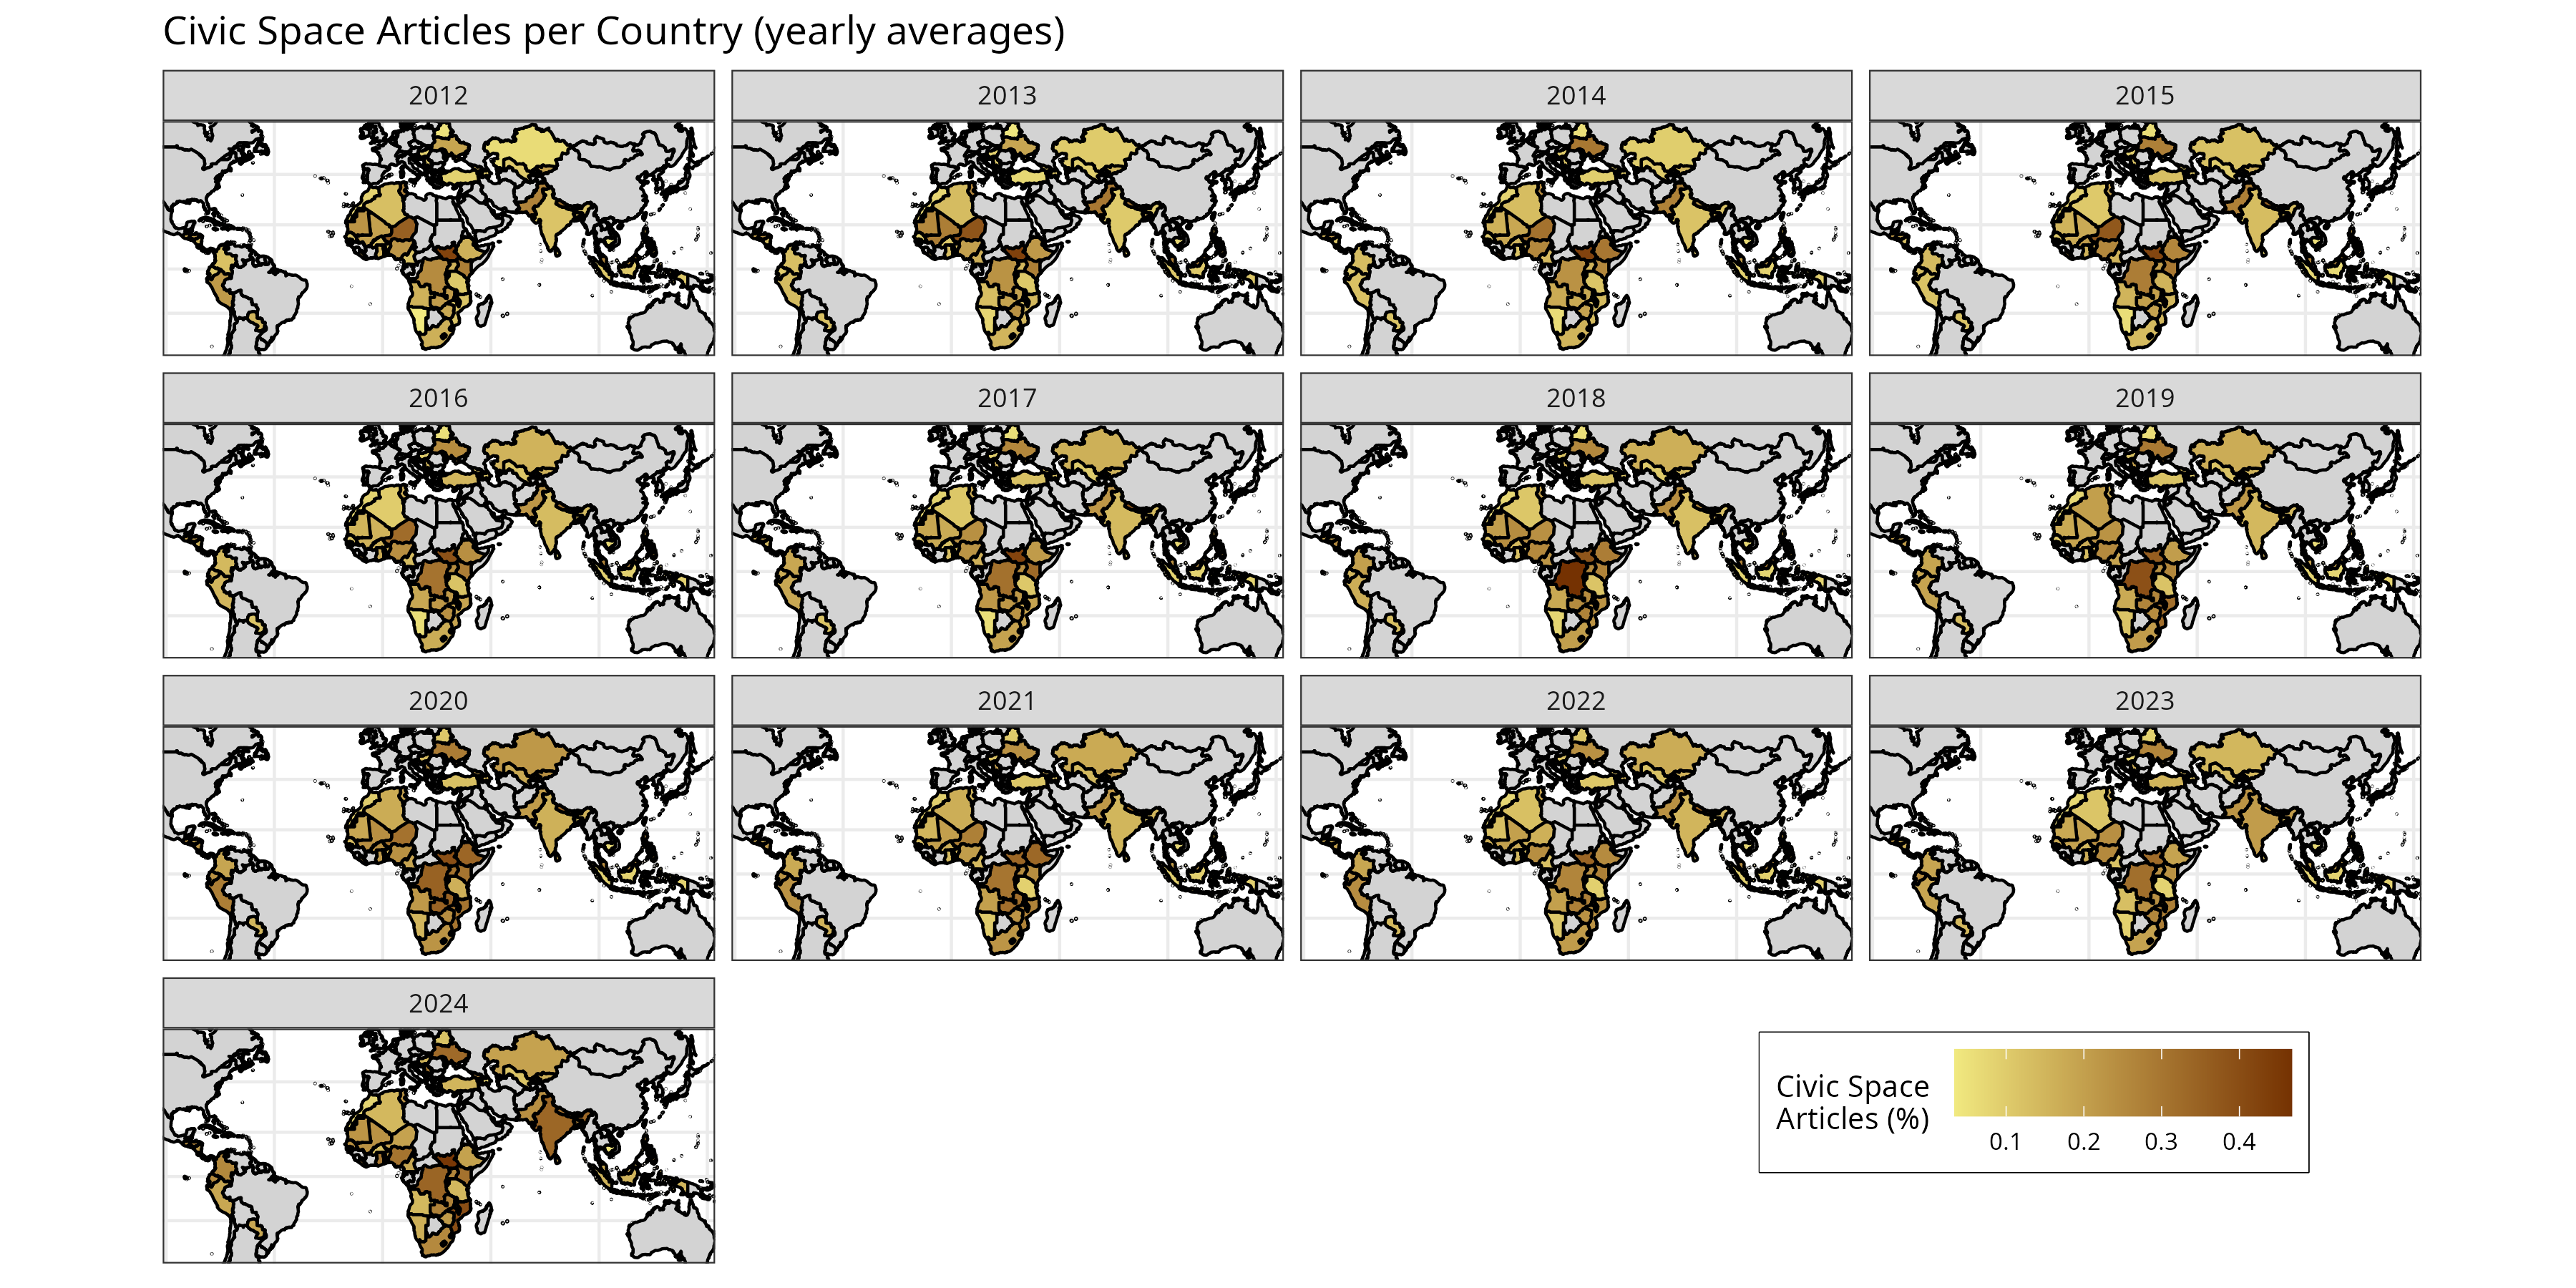
\includegraphics[width=1\linewidth,height=\textheight,keepaspectratio]{descriptive_maps/figures/civic_space_percentage_appendix.png}

}

\caption{\label{fig-civic-space-percentage}Civic space articles as
percentage of total coverage by country-year. Countries are colored
according to the proportion of their total news coverage dedicated to
civic space events, providing insight into the relative salience of
civic space issues across different national contexts. Light gray areas
indicate countries without data coverage. The maps show temporal
evolution from 2012 through 2024, revealing significant variation in
civic space reporting intensity both across countries and over time.}

\end{figure}%

\subsection{Dominant Civic Events by
Country}\label{dominant-civic-events-by-country}

\begin{figure}

\centering{

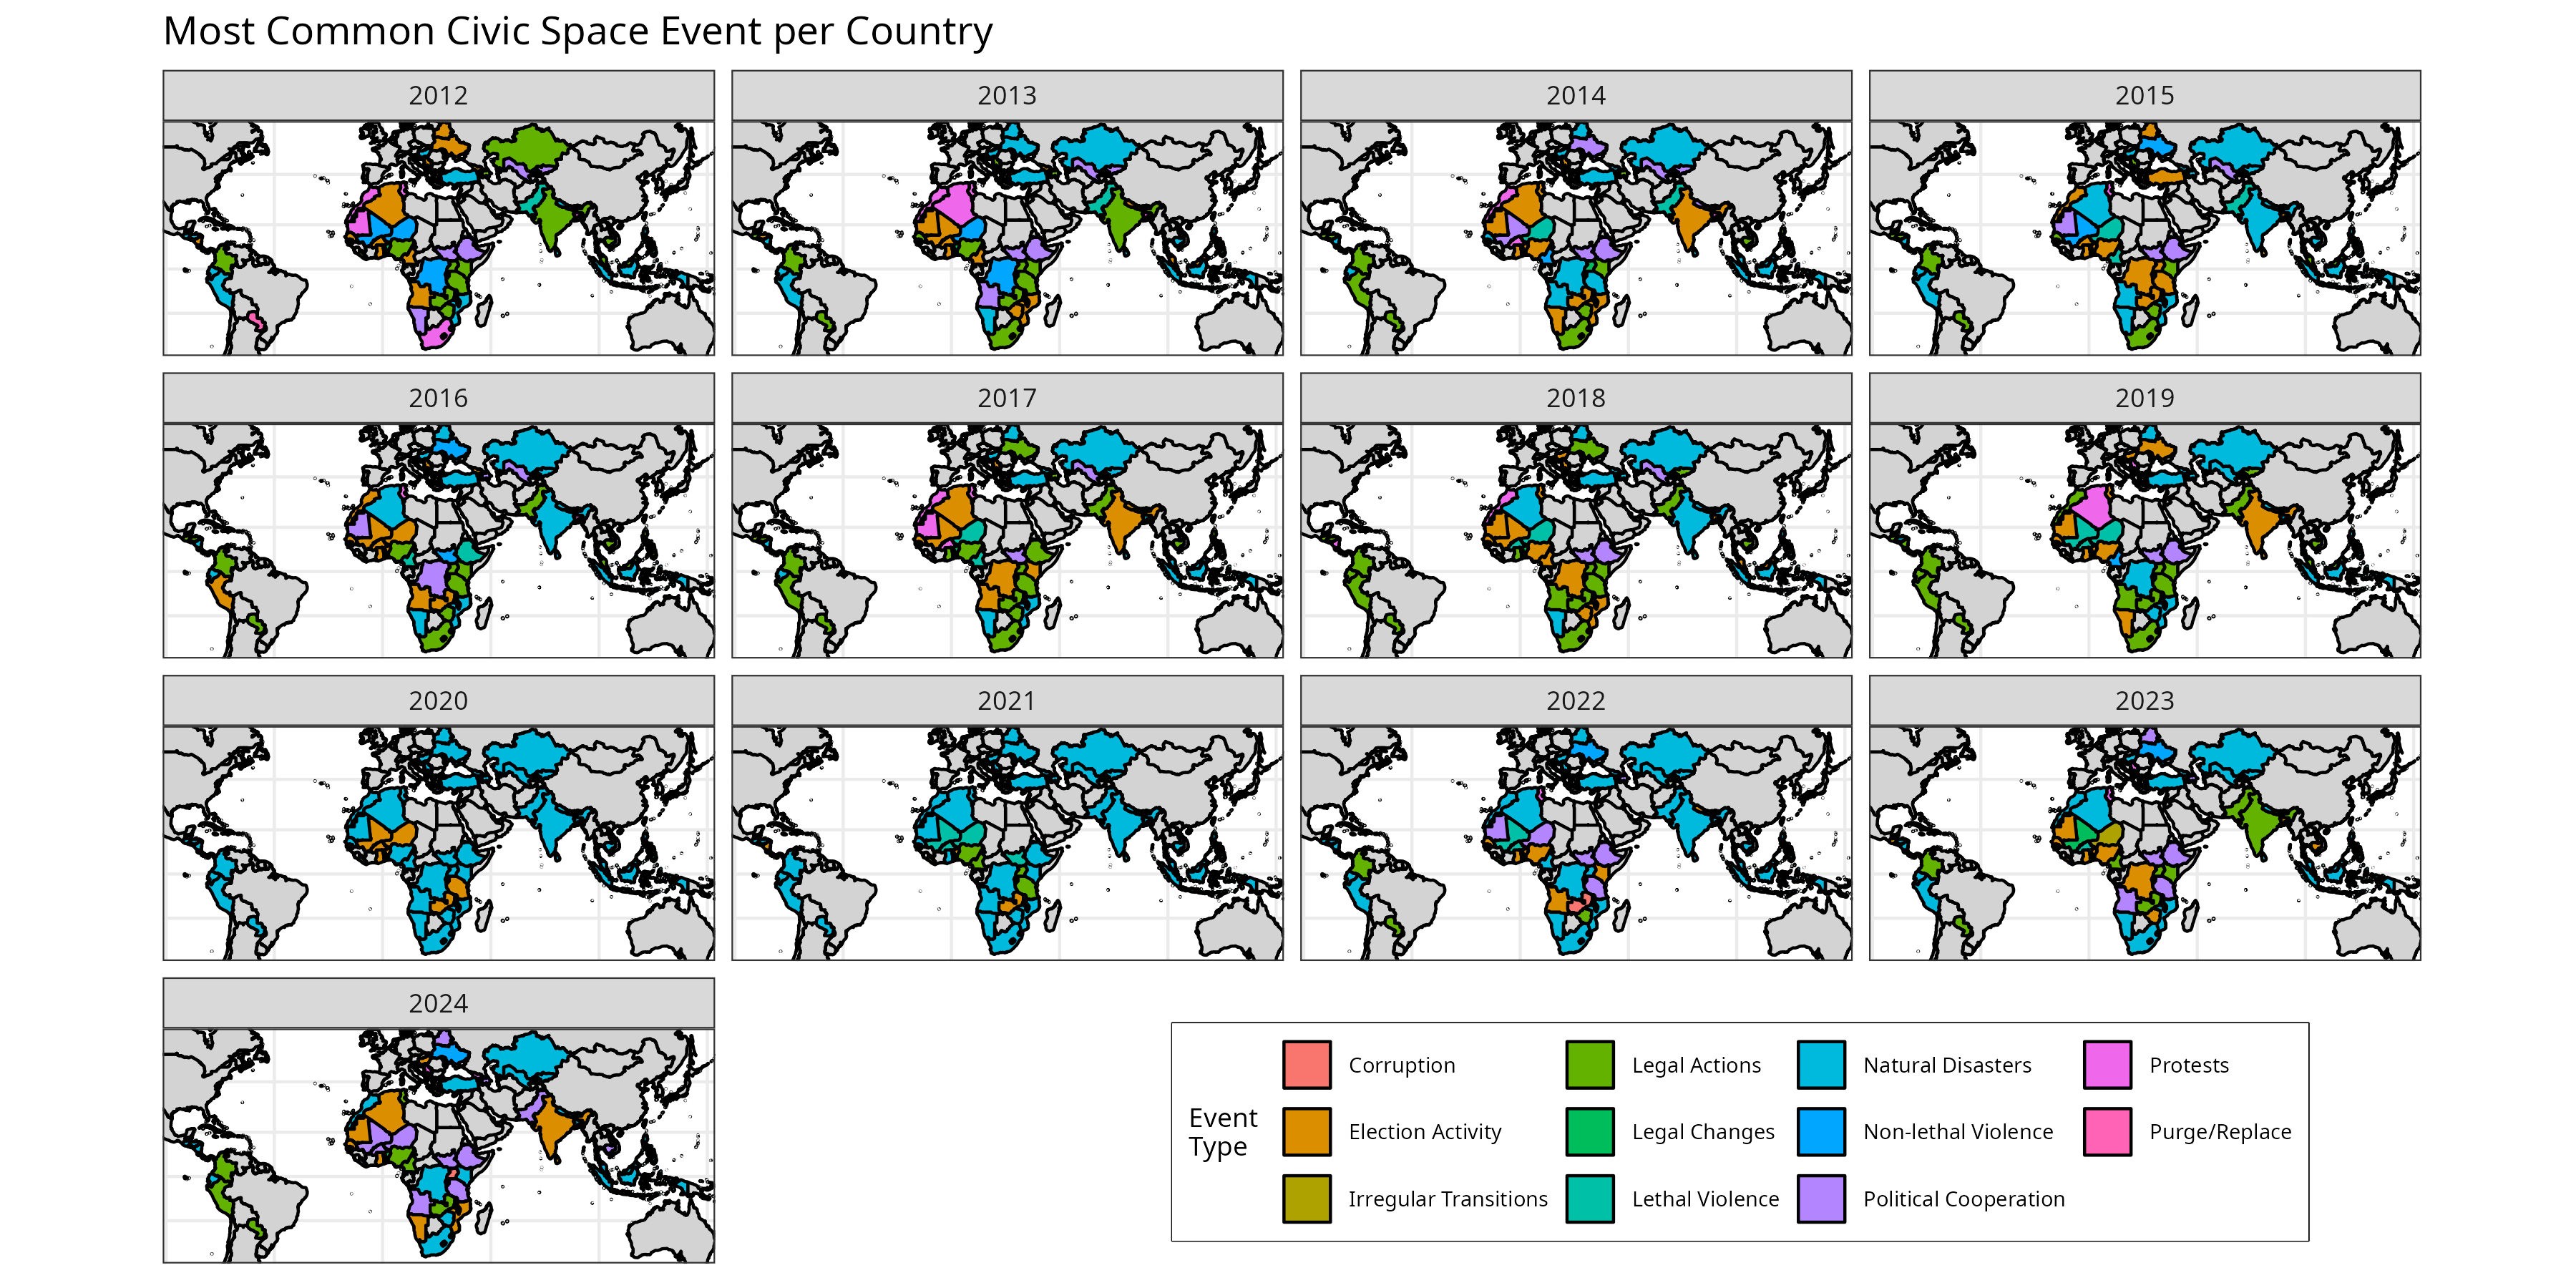
\includegraphics[width=1\linewidth,height=\textheight,keepaspectratio]{descriptive_maps/figures/dominant_event_appendix.png}

}

\caption{\label{fig-dominant-events}Most frequently reported civic event
type per country-year. Countries are colored according to the civic
event category with the highest reporting frequency in each year,
showing the diversity of civic space concerns across different national
contexts. The maps reveal regional patterns in dominant event types and
temporal shifts in civic space priorities, from electoral activities to
protests, corruption reporting, and other civic engagement forms.}

\end{figure}%

\section{Appendix D: Validation
Figures}\label{appendix-d-validation-figures}

These validation figures demonstrate the effectiveness of ML4P's event
detection methodology by examining State of Emergency declarations
across different regions during the COVID-19 pandemic. The vertical
dashed red line at March 2020 marks the onset of the global pandemic,
when countries worldwide implemented emergency measures including
lockdowns, curfews, and restrictions on civil liberties. These plots
validate our approach by showing systematic spikes in State of Emergency
reporting across all regions coinciding with known policy responses to
the pandemic.

\subsection{State of Emergency Detection by
Region}\label{state-of-emergency-detection-by-region}

\begin{figure}

\centering{

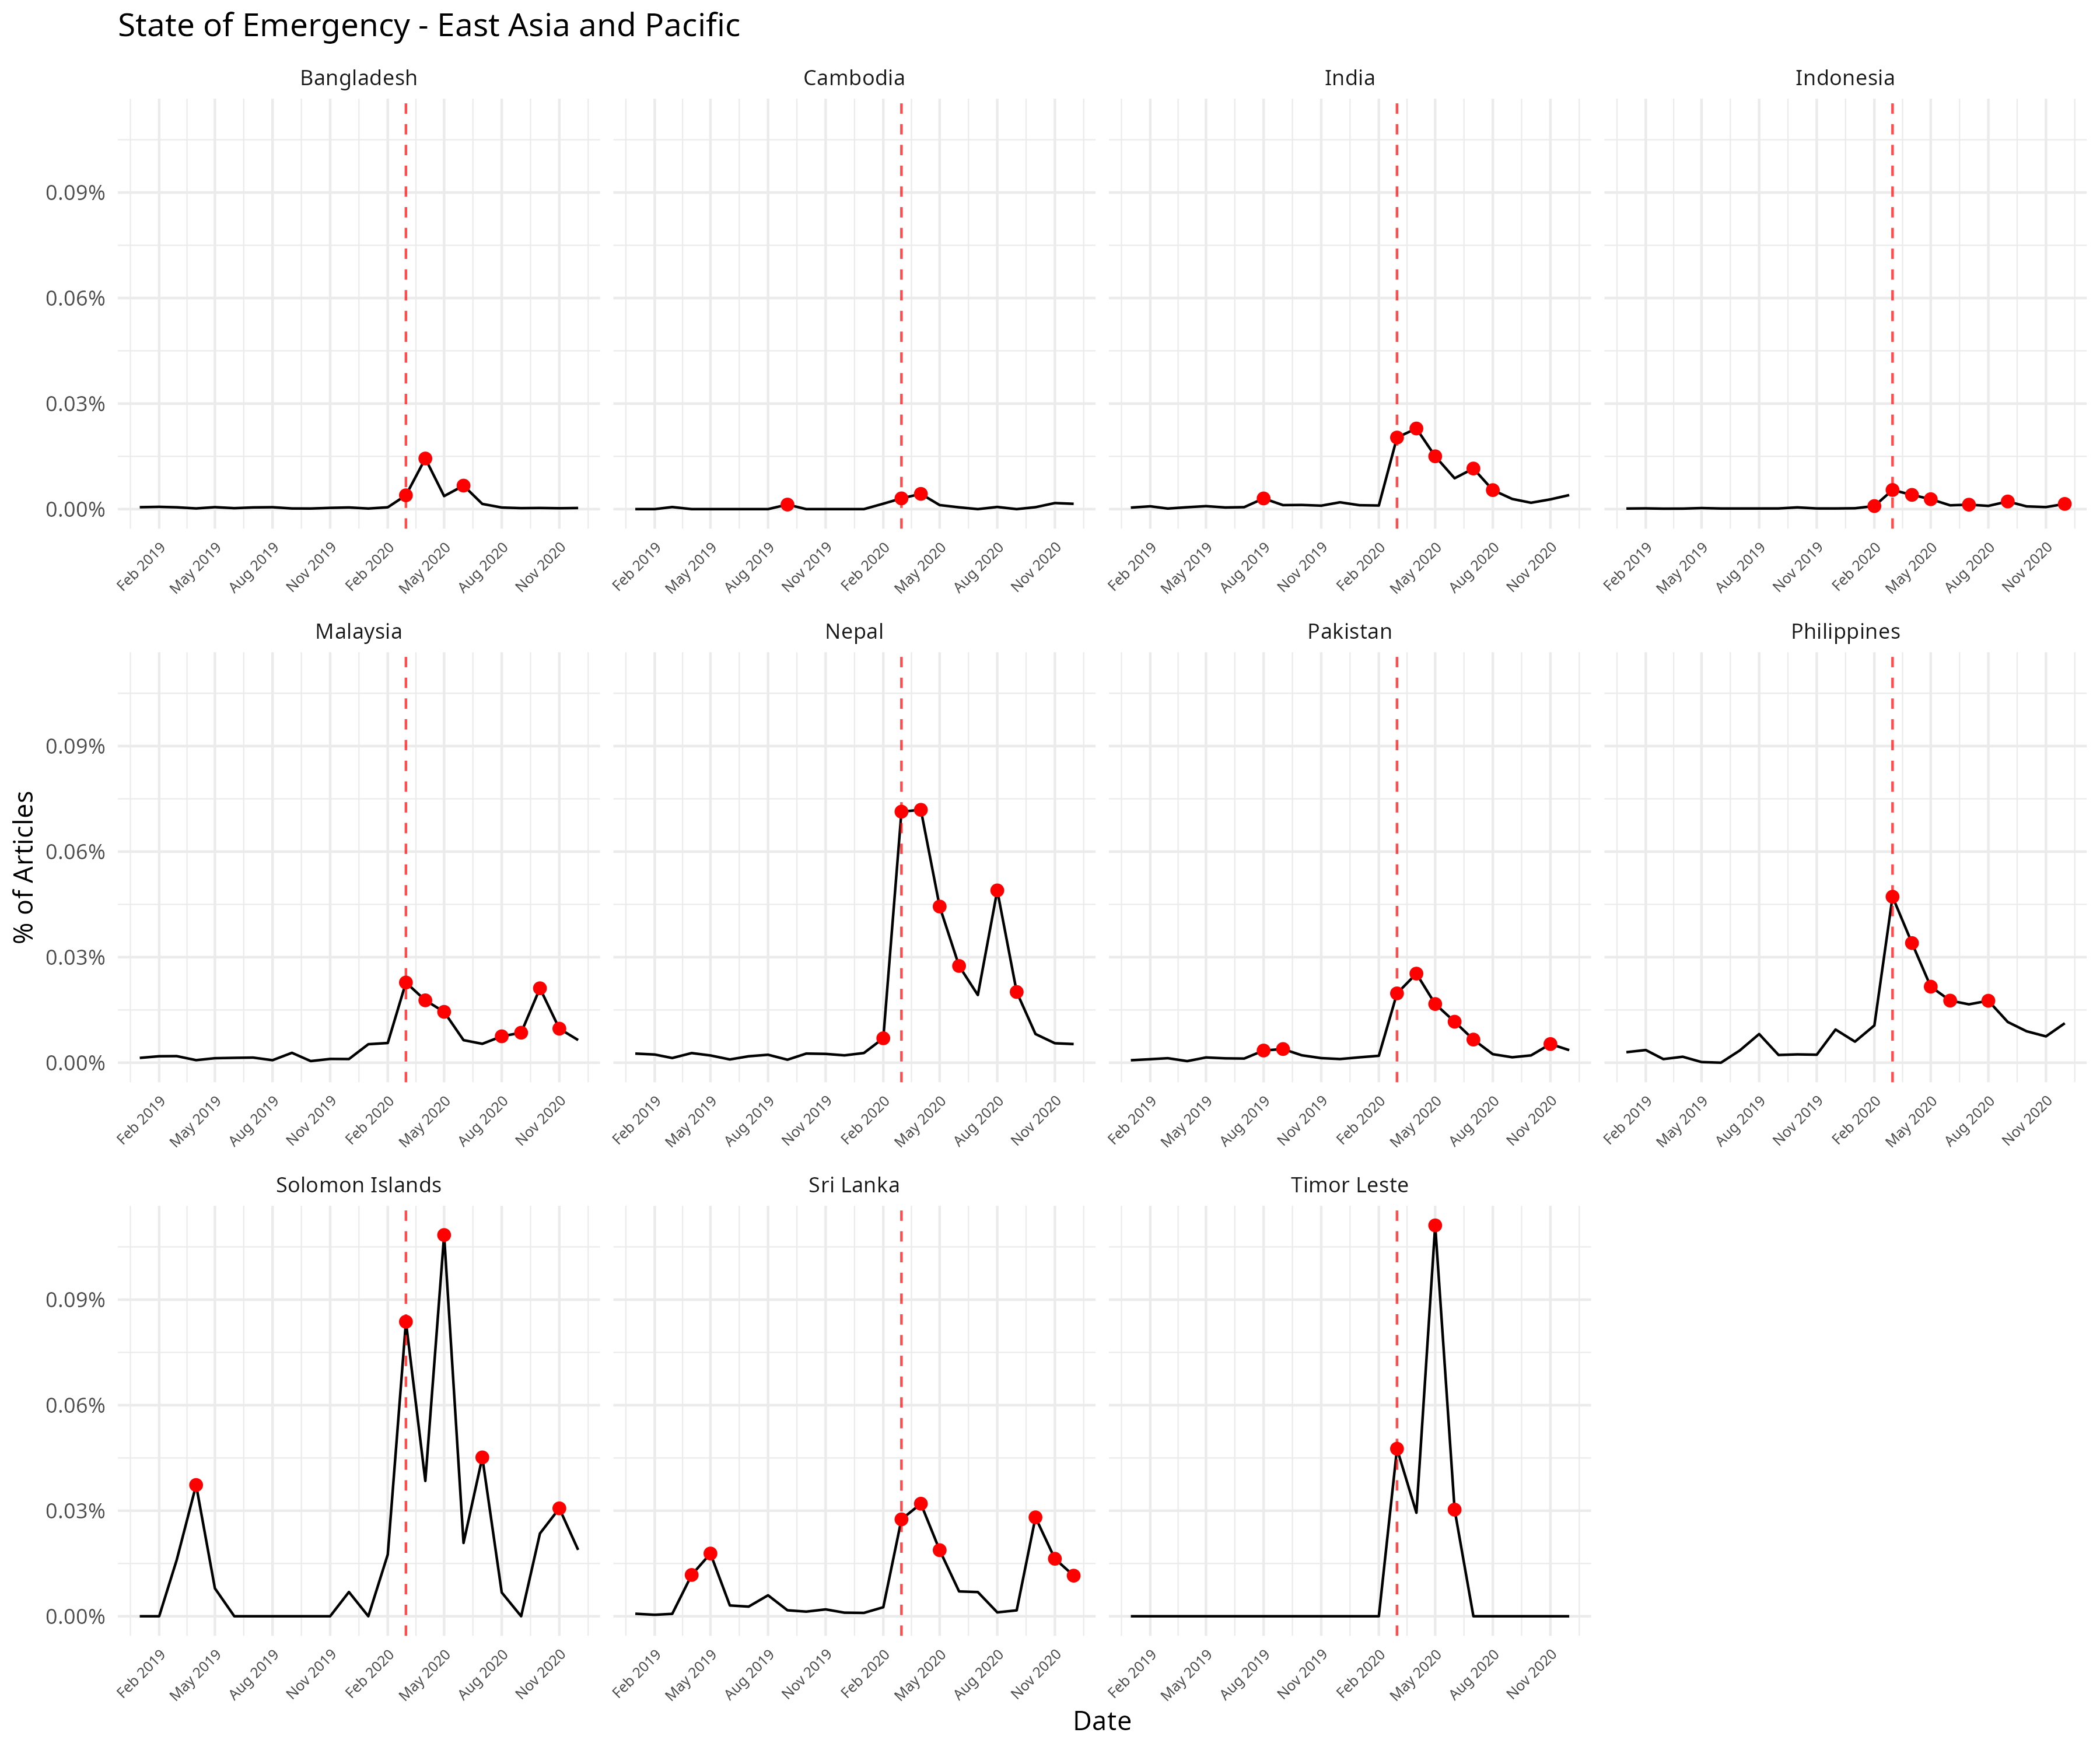
\includegraphics[width=1\linewidth,height=\textheight,keepaspectratio]{event_validation/State_of_Emergency_East_Asia_and_Pacific.png}

}

\caption{\label{fig-soe-eap}State of Emergency events detection in East
Asia and Pacific countries from 2019-2020. The plot shows the percentage
of articles devoted to State of Emergency coverage over time, with red
points indicating detected shock events. The vertical dashed red line
marks March 2020, the beginning of the COVID-19 pandemic. Clear spikes
are visible across multiple countries starting in March 2020,
corresponding to the implementation of emergency measures and lockdowns
in response to the pandemic.}

\end{figure}%

\begin{figure}

\centering{

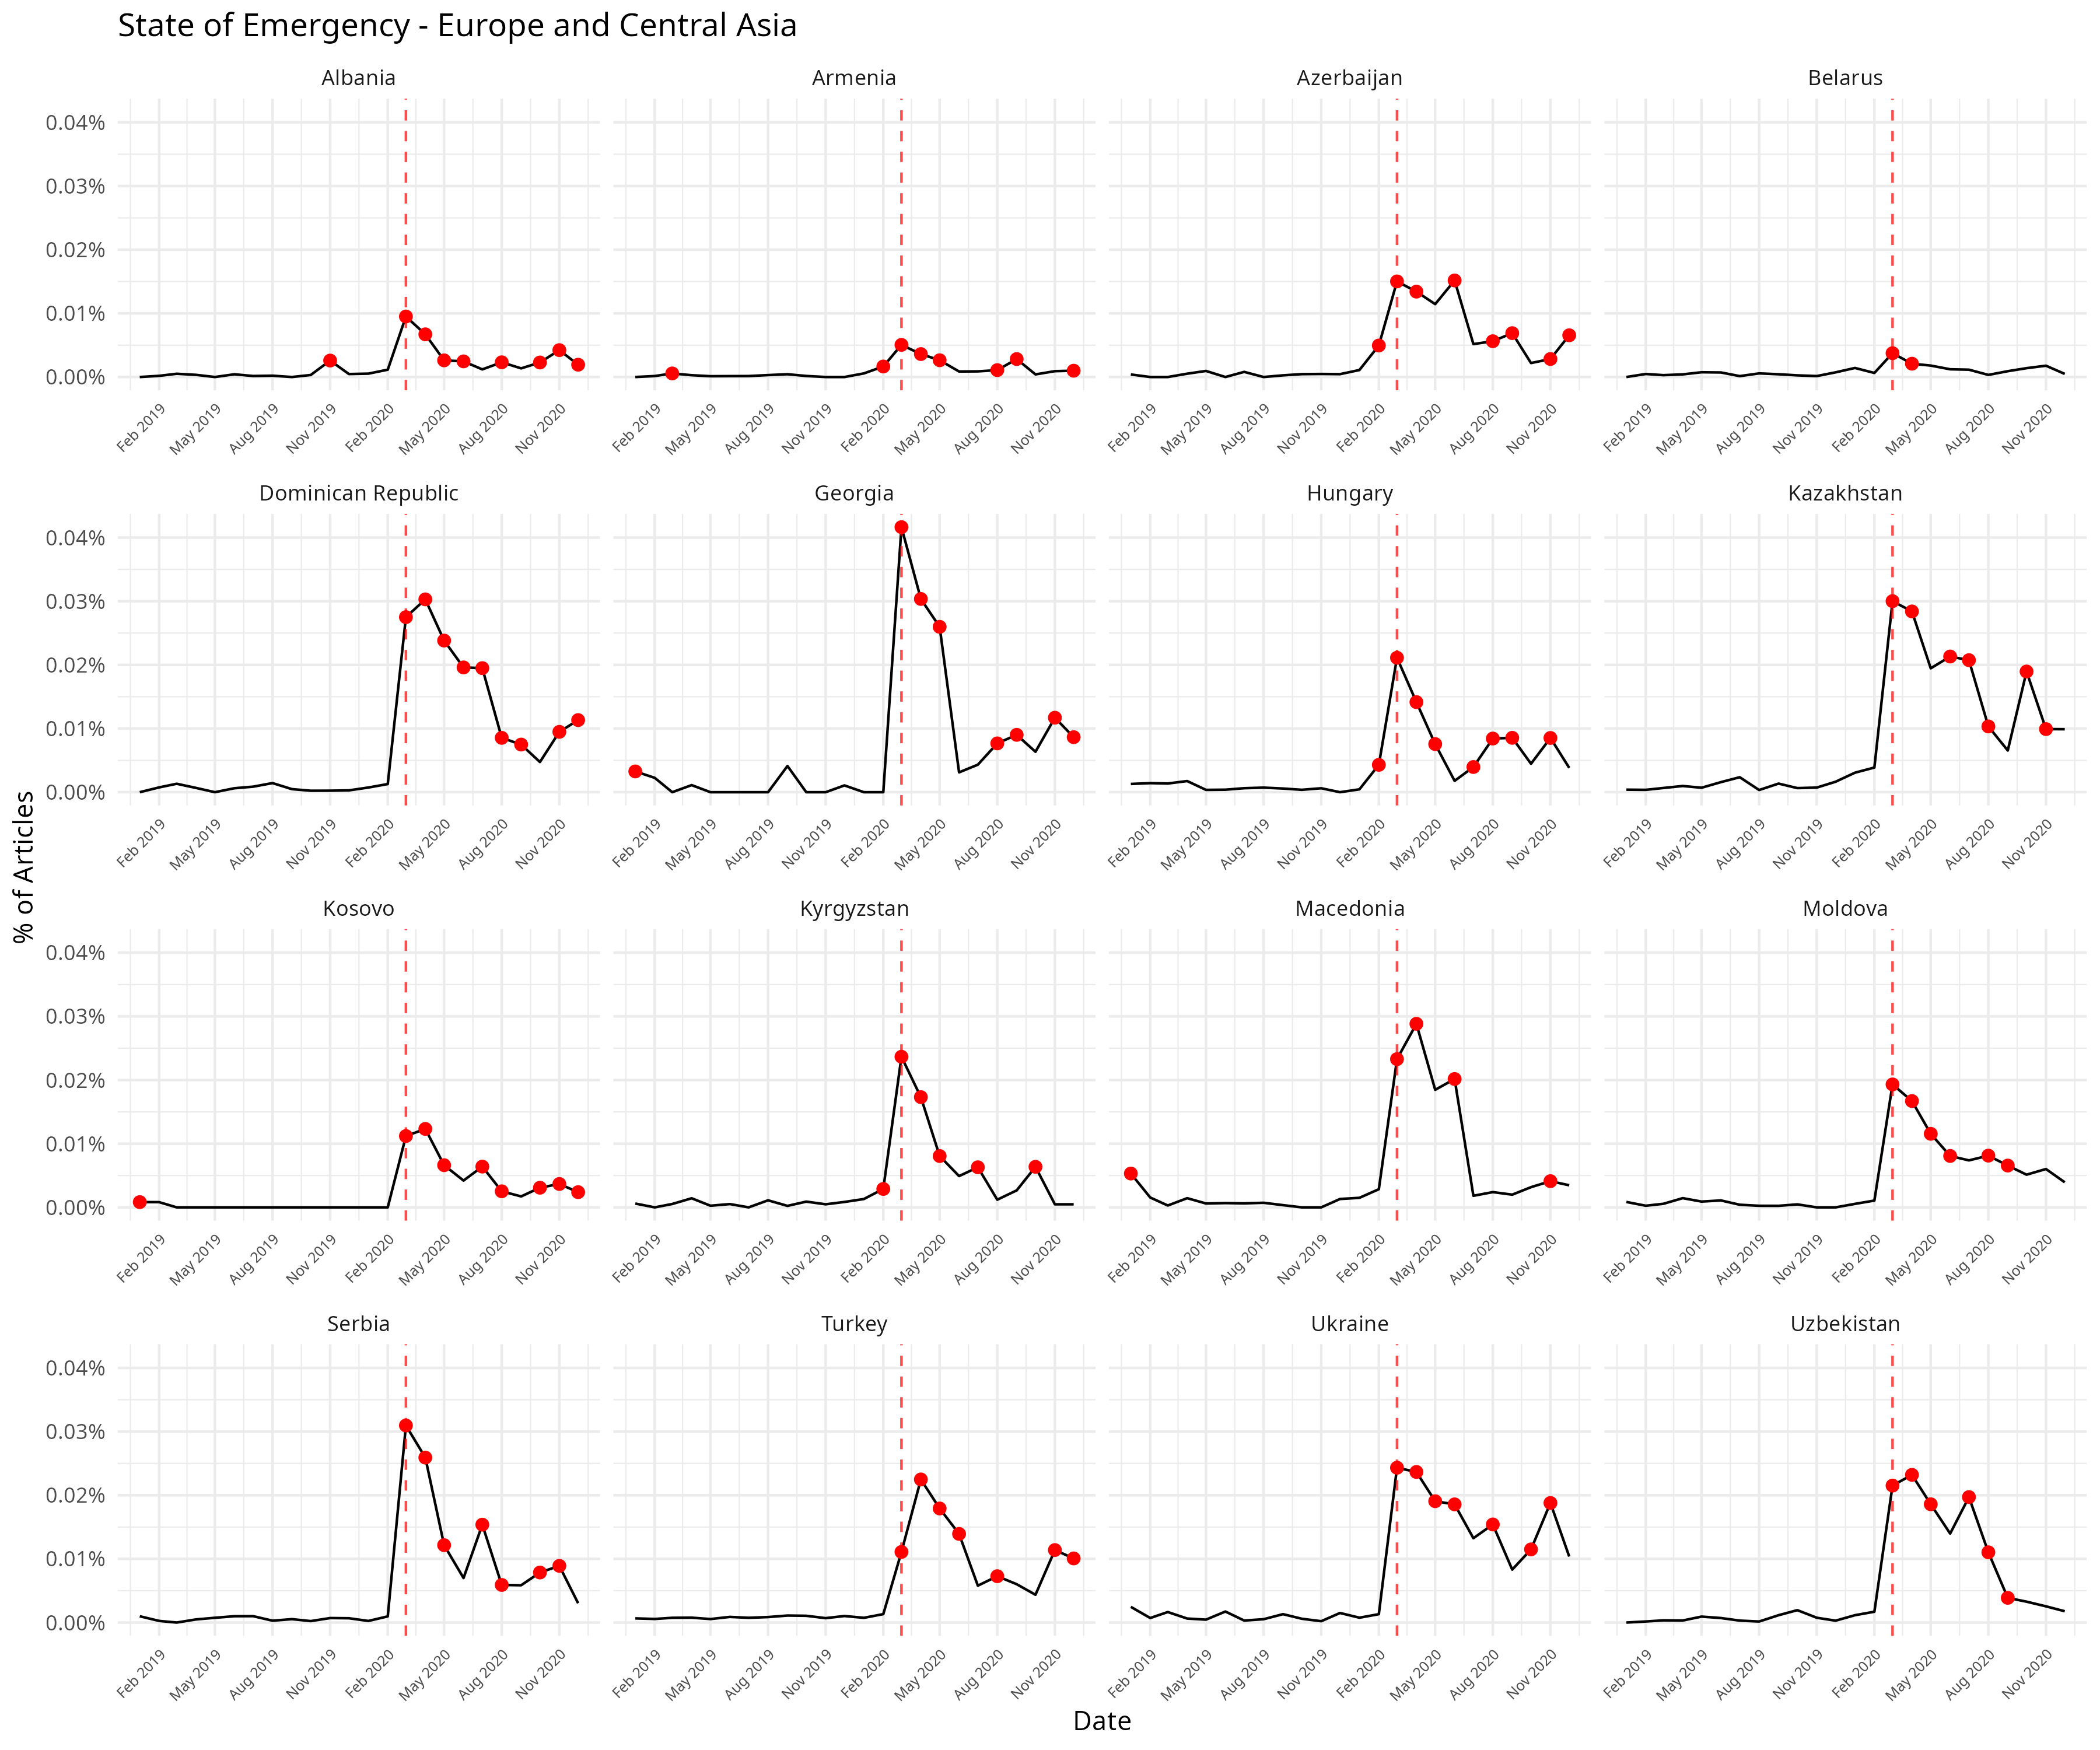
\includegraphics[width=1\linewidth,height=\textheight,keepaspectratio]{event_validation/State_of_Emergency_Europe_and_Central_Asia.png}

}

\caption{\label{fig-soe-eca}State of Emergency events detection in
Europe and Central Asia countries from 2019-2020. The plot shows the
percentage of articles devoted to State of Emergency coverage over time,
with red points indicating detected shock events. The vertical dashed
red line marks March 2020, the beginning of the COVID-19 pandemic.
Pronounced spikes are evident across the region starting in March 2020,
reflecting the widespread implementation of emergency measures in
response to the pandemic.}

\end{figure}%

\begin{figure}

\centering{

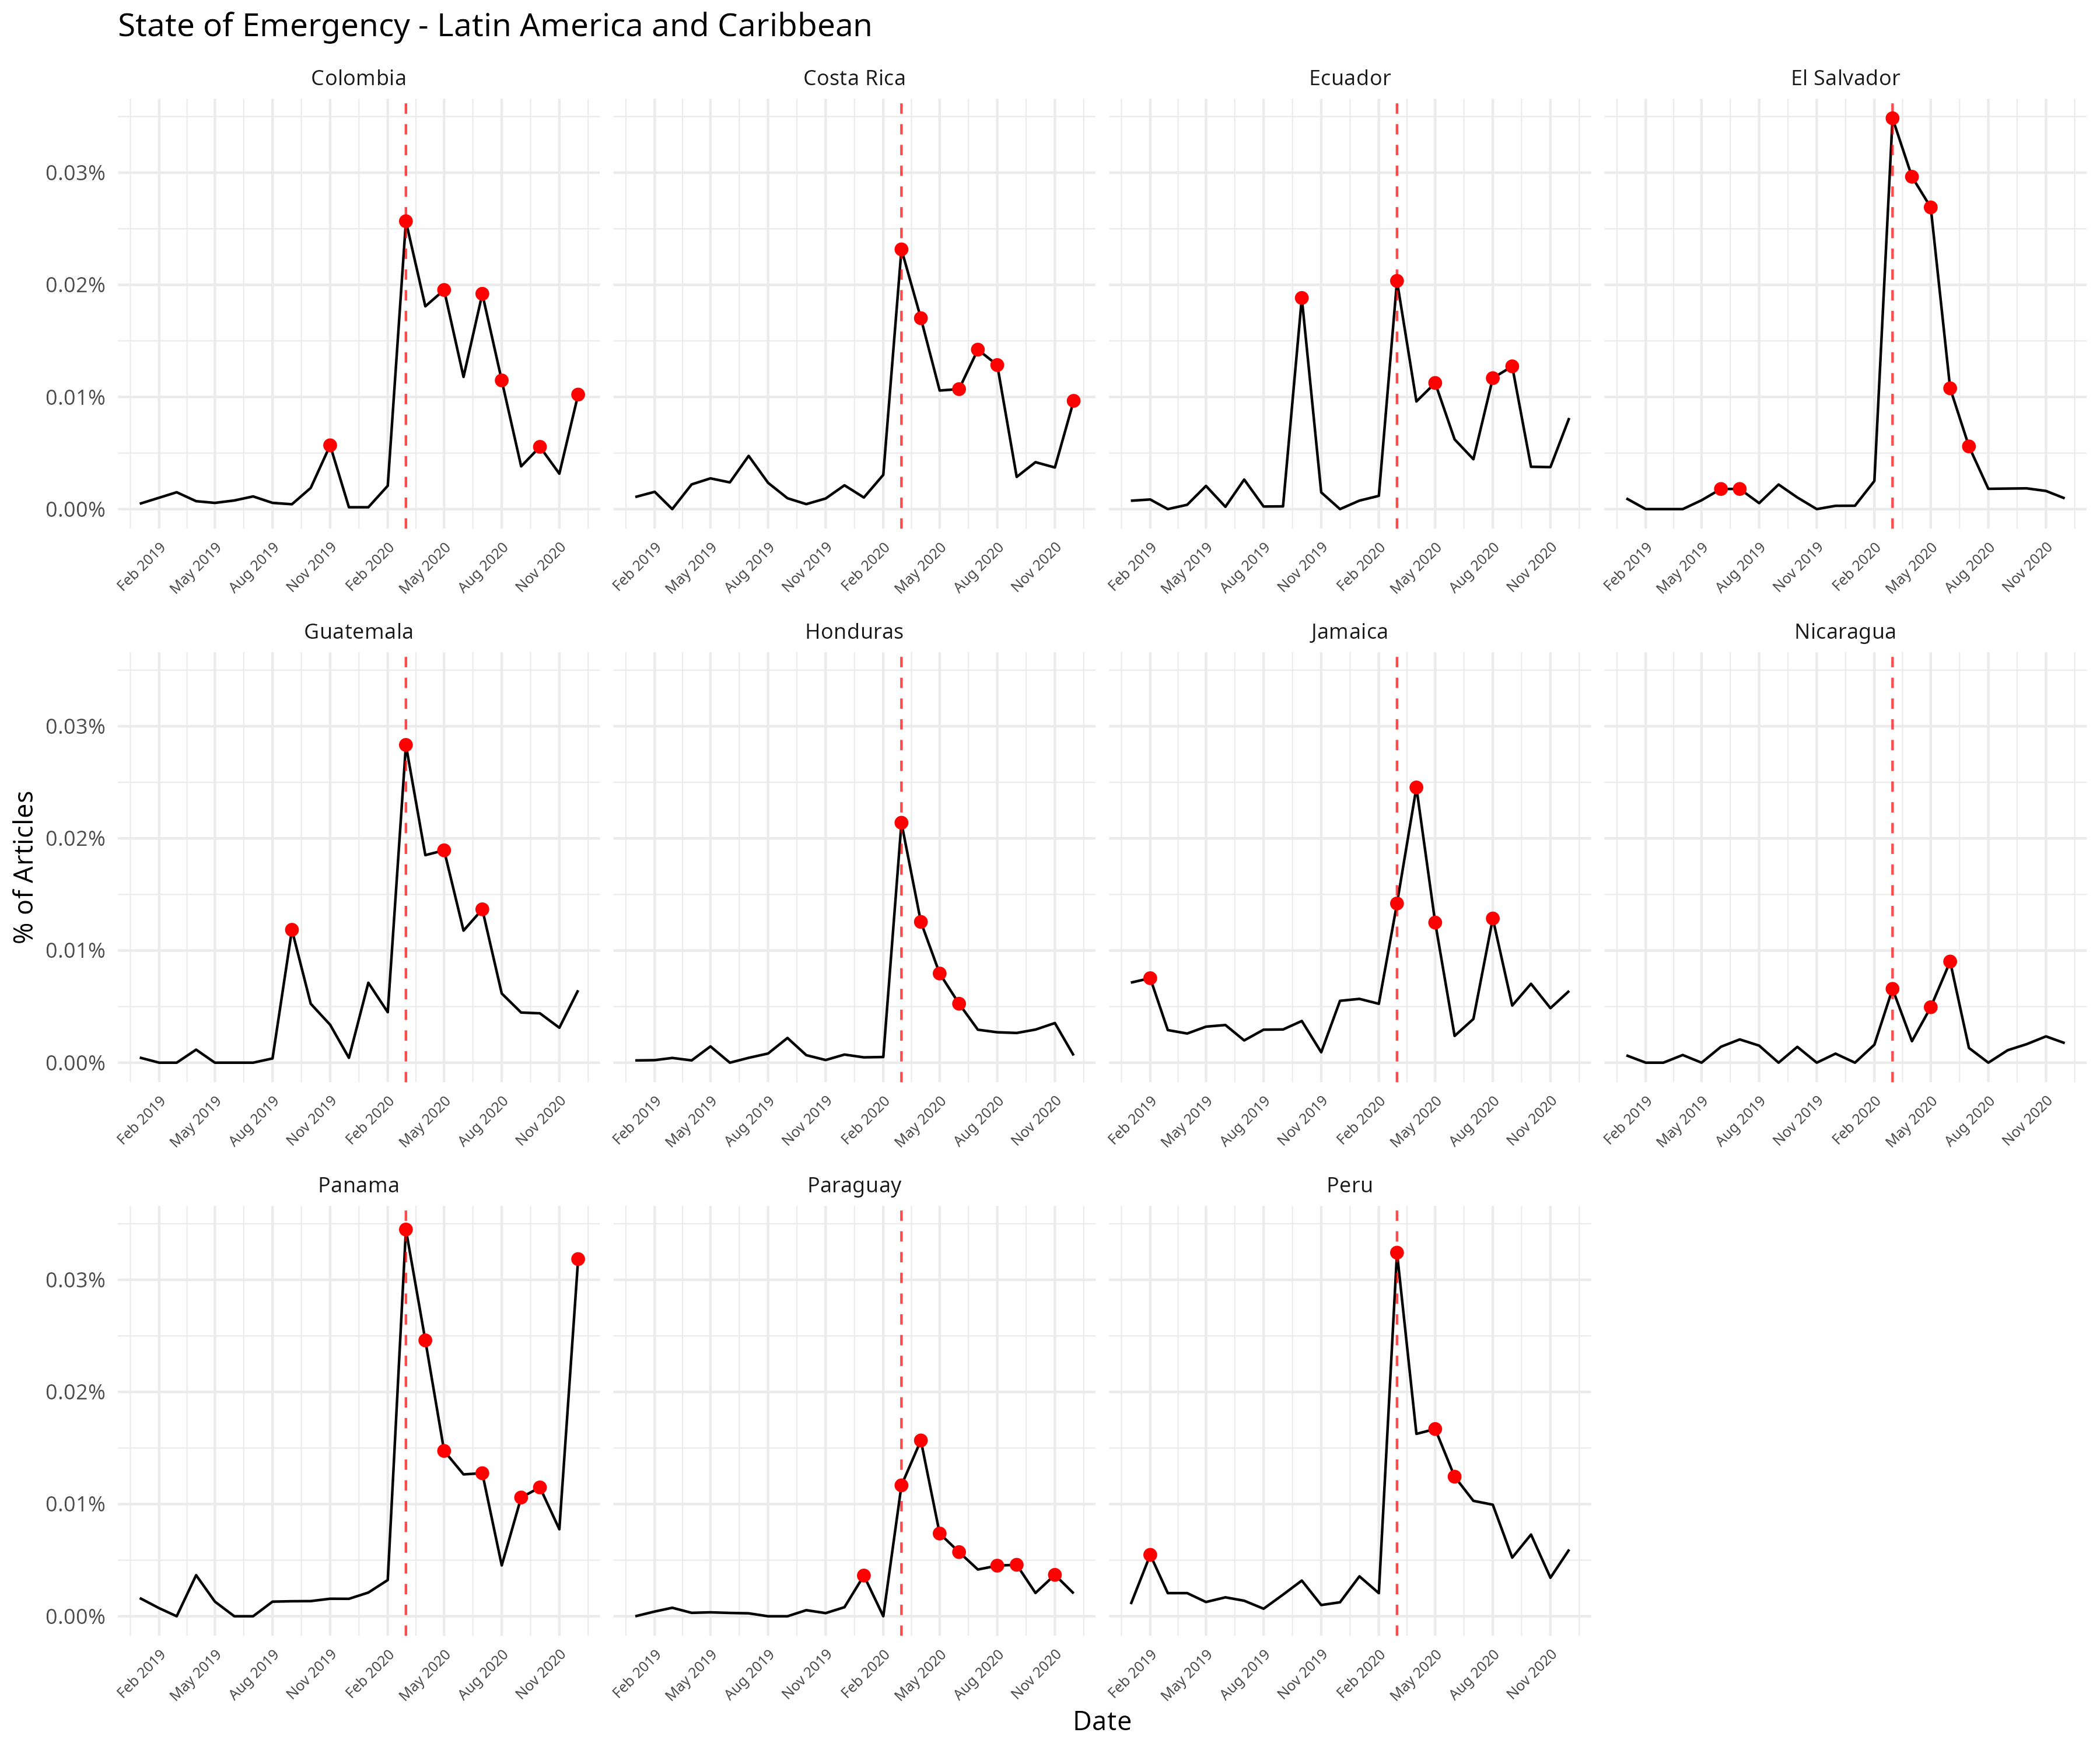
\includegraphics[width=1\linewidth,height=\textheight,keepaspectratio]{event_validation/State_of_Emergency_Latin_America_and_Caribbean.png}

}

\caption{\label{fig-soe-lac}State of Emergency events detection in Latin
America and Caribbean countries from 2019-2020. The plot shows the
percentage of articles devoted to State of Emergency coverage over time,
with red points indicating detected shock events. The vertical dashed
red line marks March 2020, the beginning of the COVID-19 pandemic.
Significant increases in State of Emergency reporting are visible across
the region starting in March 2020, corresponding to the implementation
of pandemic-related emergency measures.}

\end{figure}%

\begin{figure}

\centering{

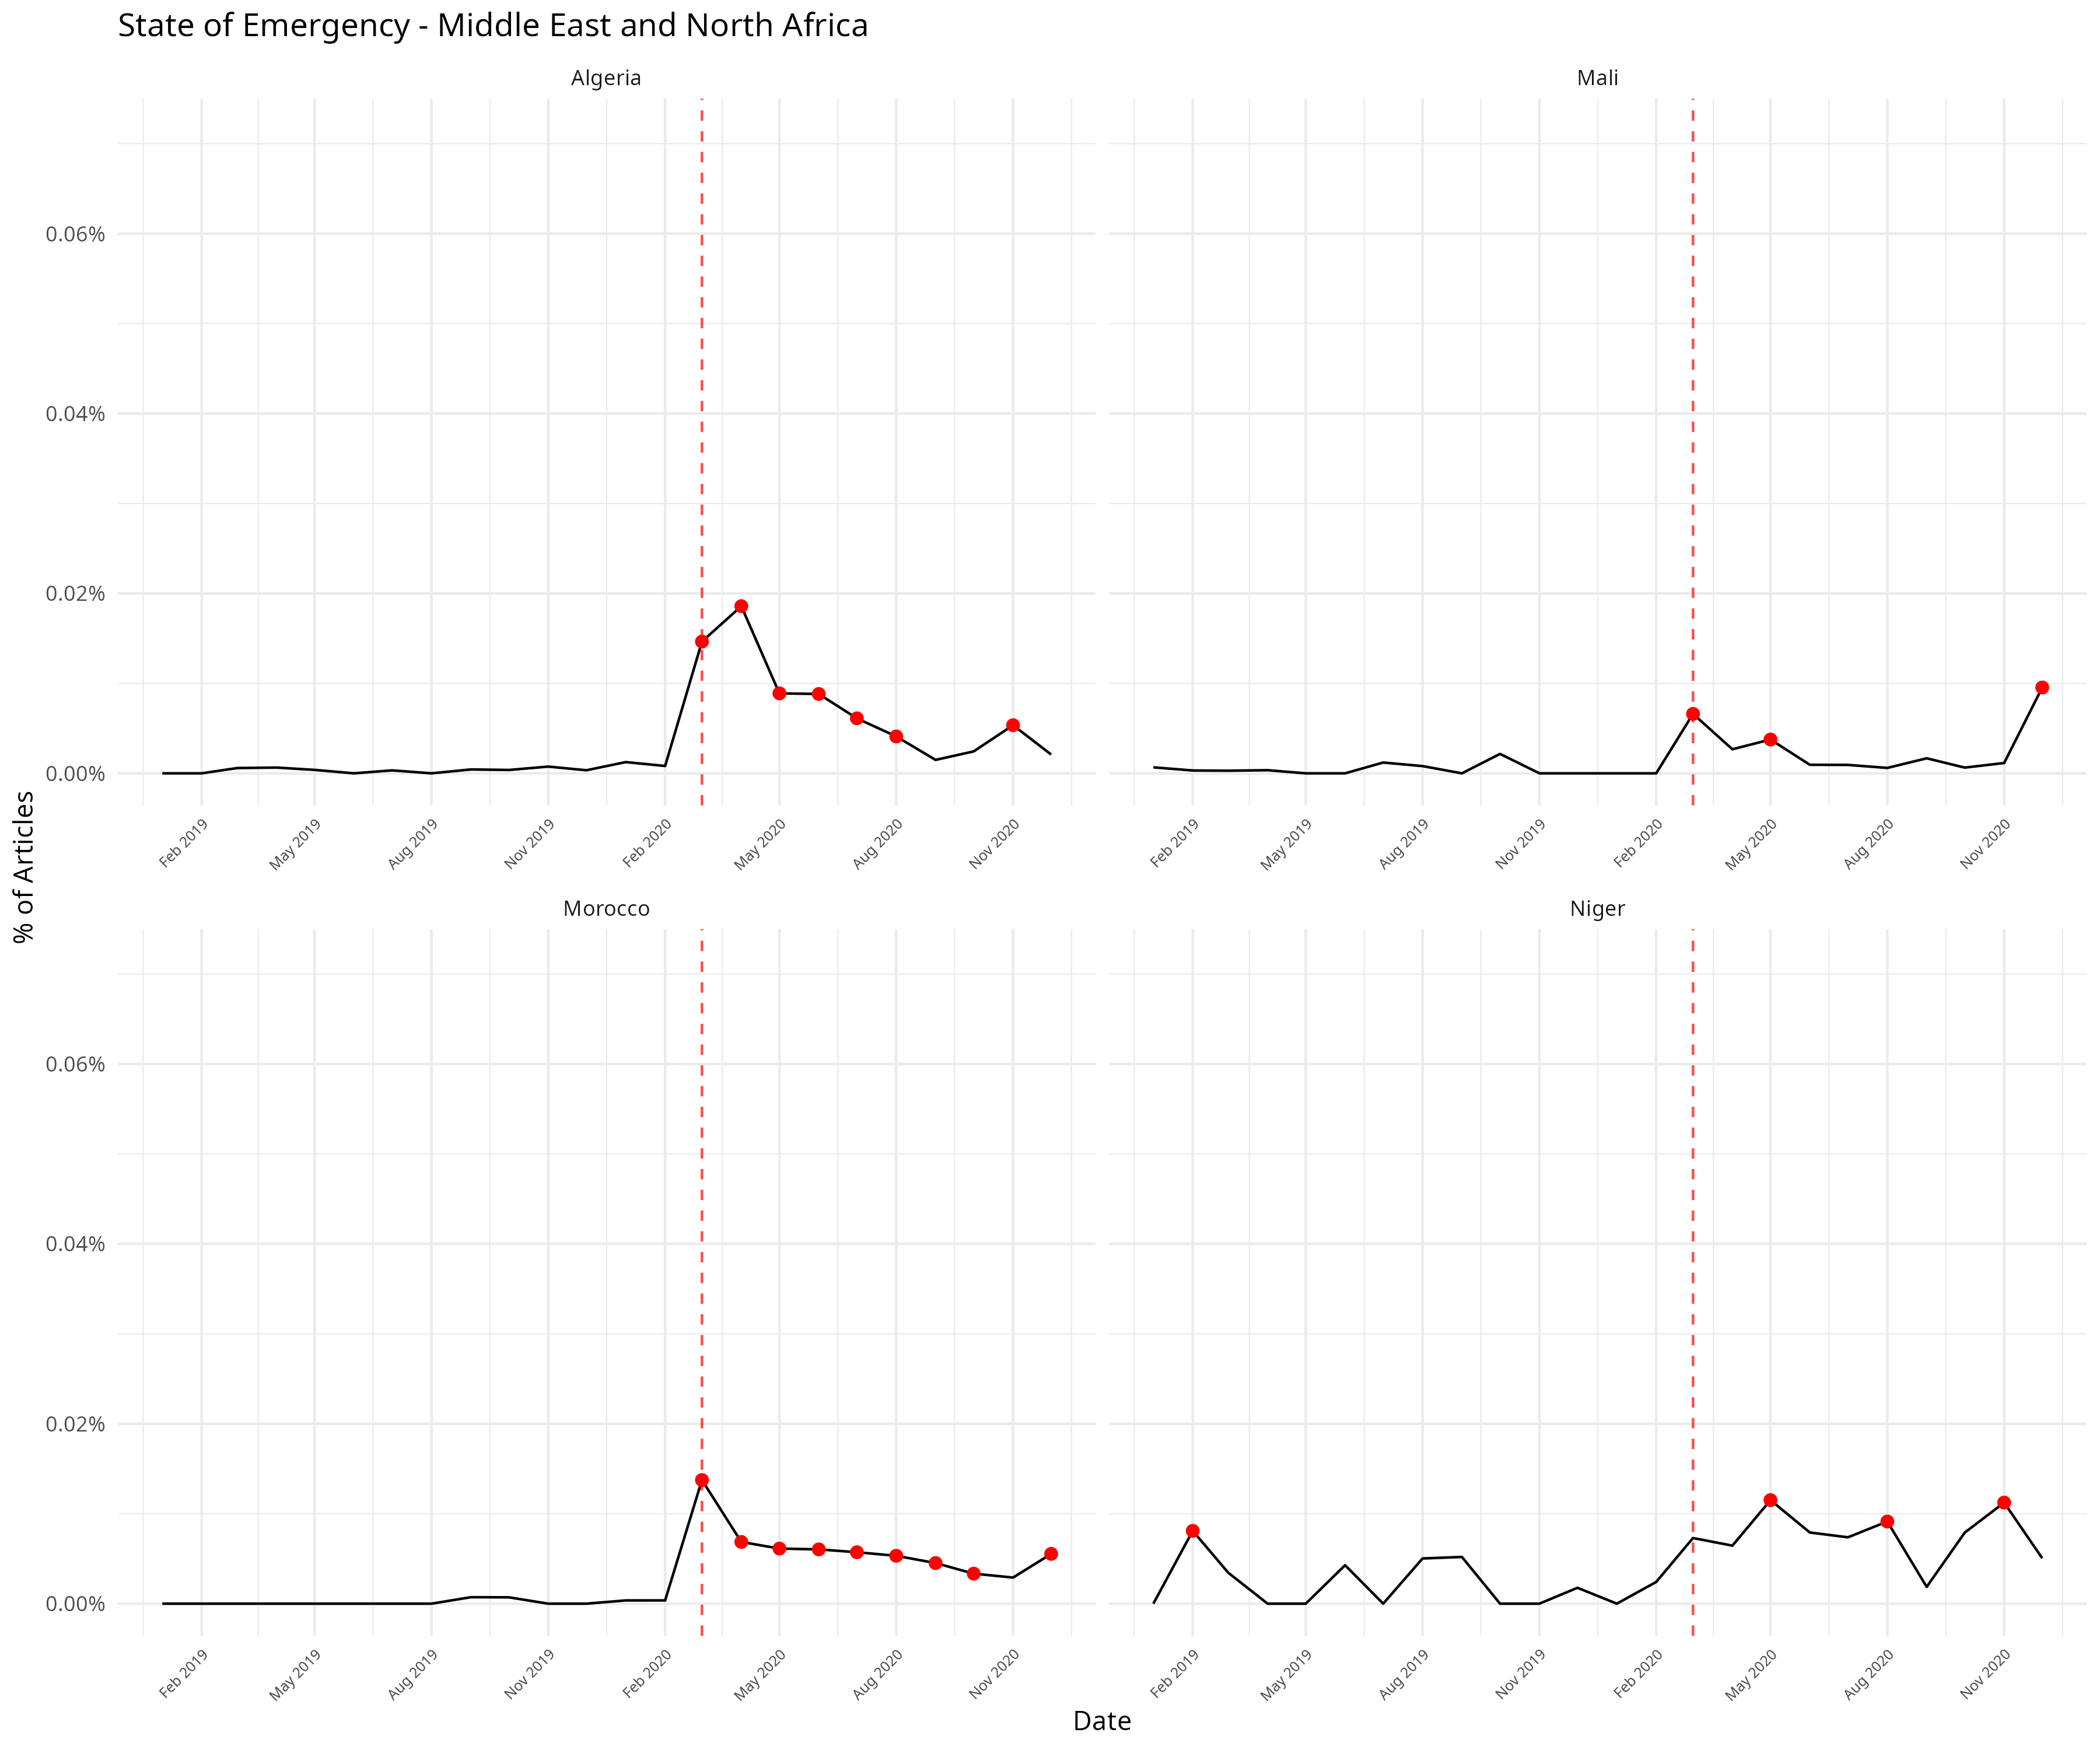
\includegraphics[width=1\linewidth,height=\textheight,keepaspectratio]{event_validation/State_of_Emergency_Middle_East_and_North_Africa.png}

}

\caption{\label{fig-soe-mena}State of Emergency events detection in
Middle East and North Africa countries from 2019-2020. The plot shows
the percentage of articles devoted to State of Emergency coverage over
time, with red points indicating detected shock events. The vertical
dashed red line marks March 2020, the beginning of the COVID-19
pandemic. Clear spikes in State of Emergency reporting are visible
across countries in the region starting in March 2020, reflecting the
implementation of emergency measures in response to the pandemic.}

\end{figure}%

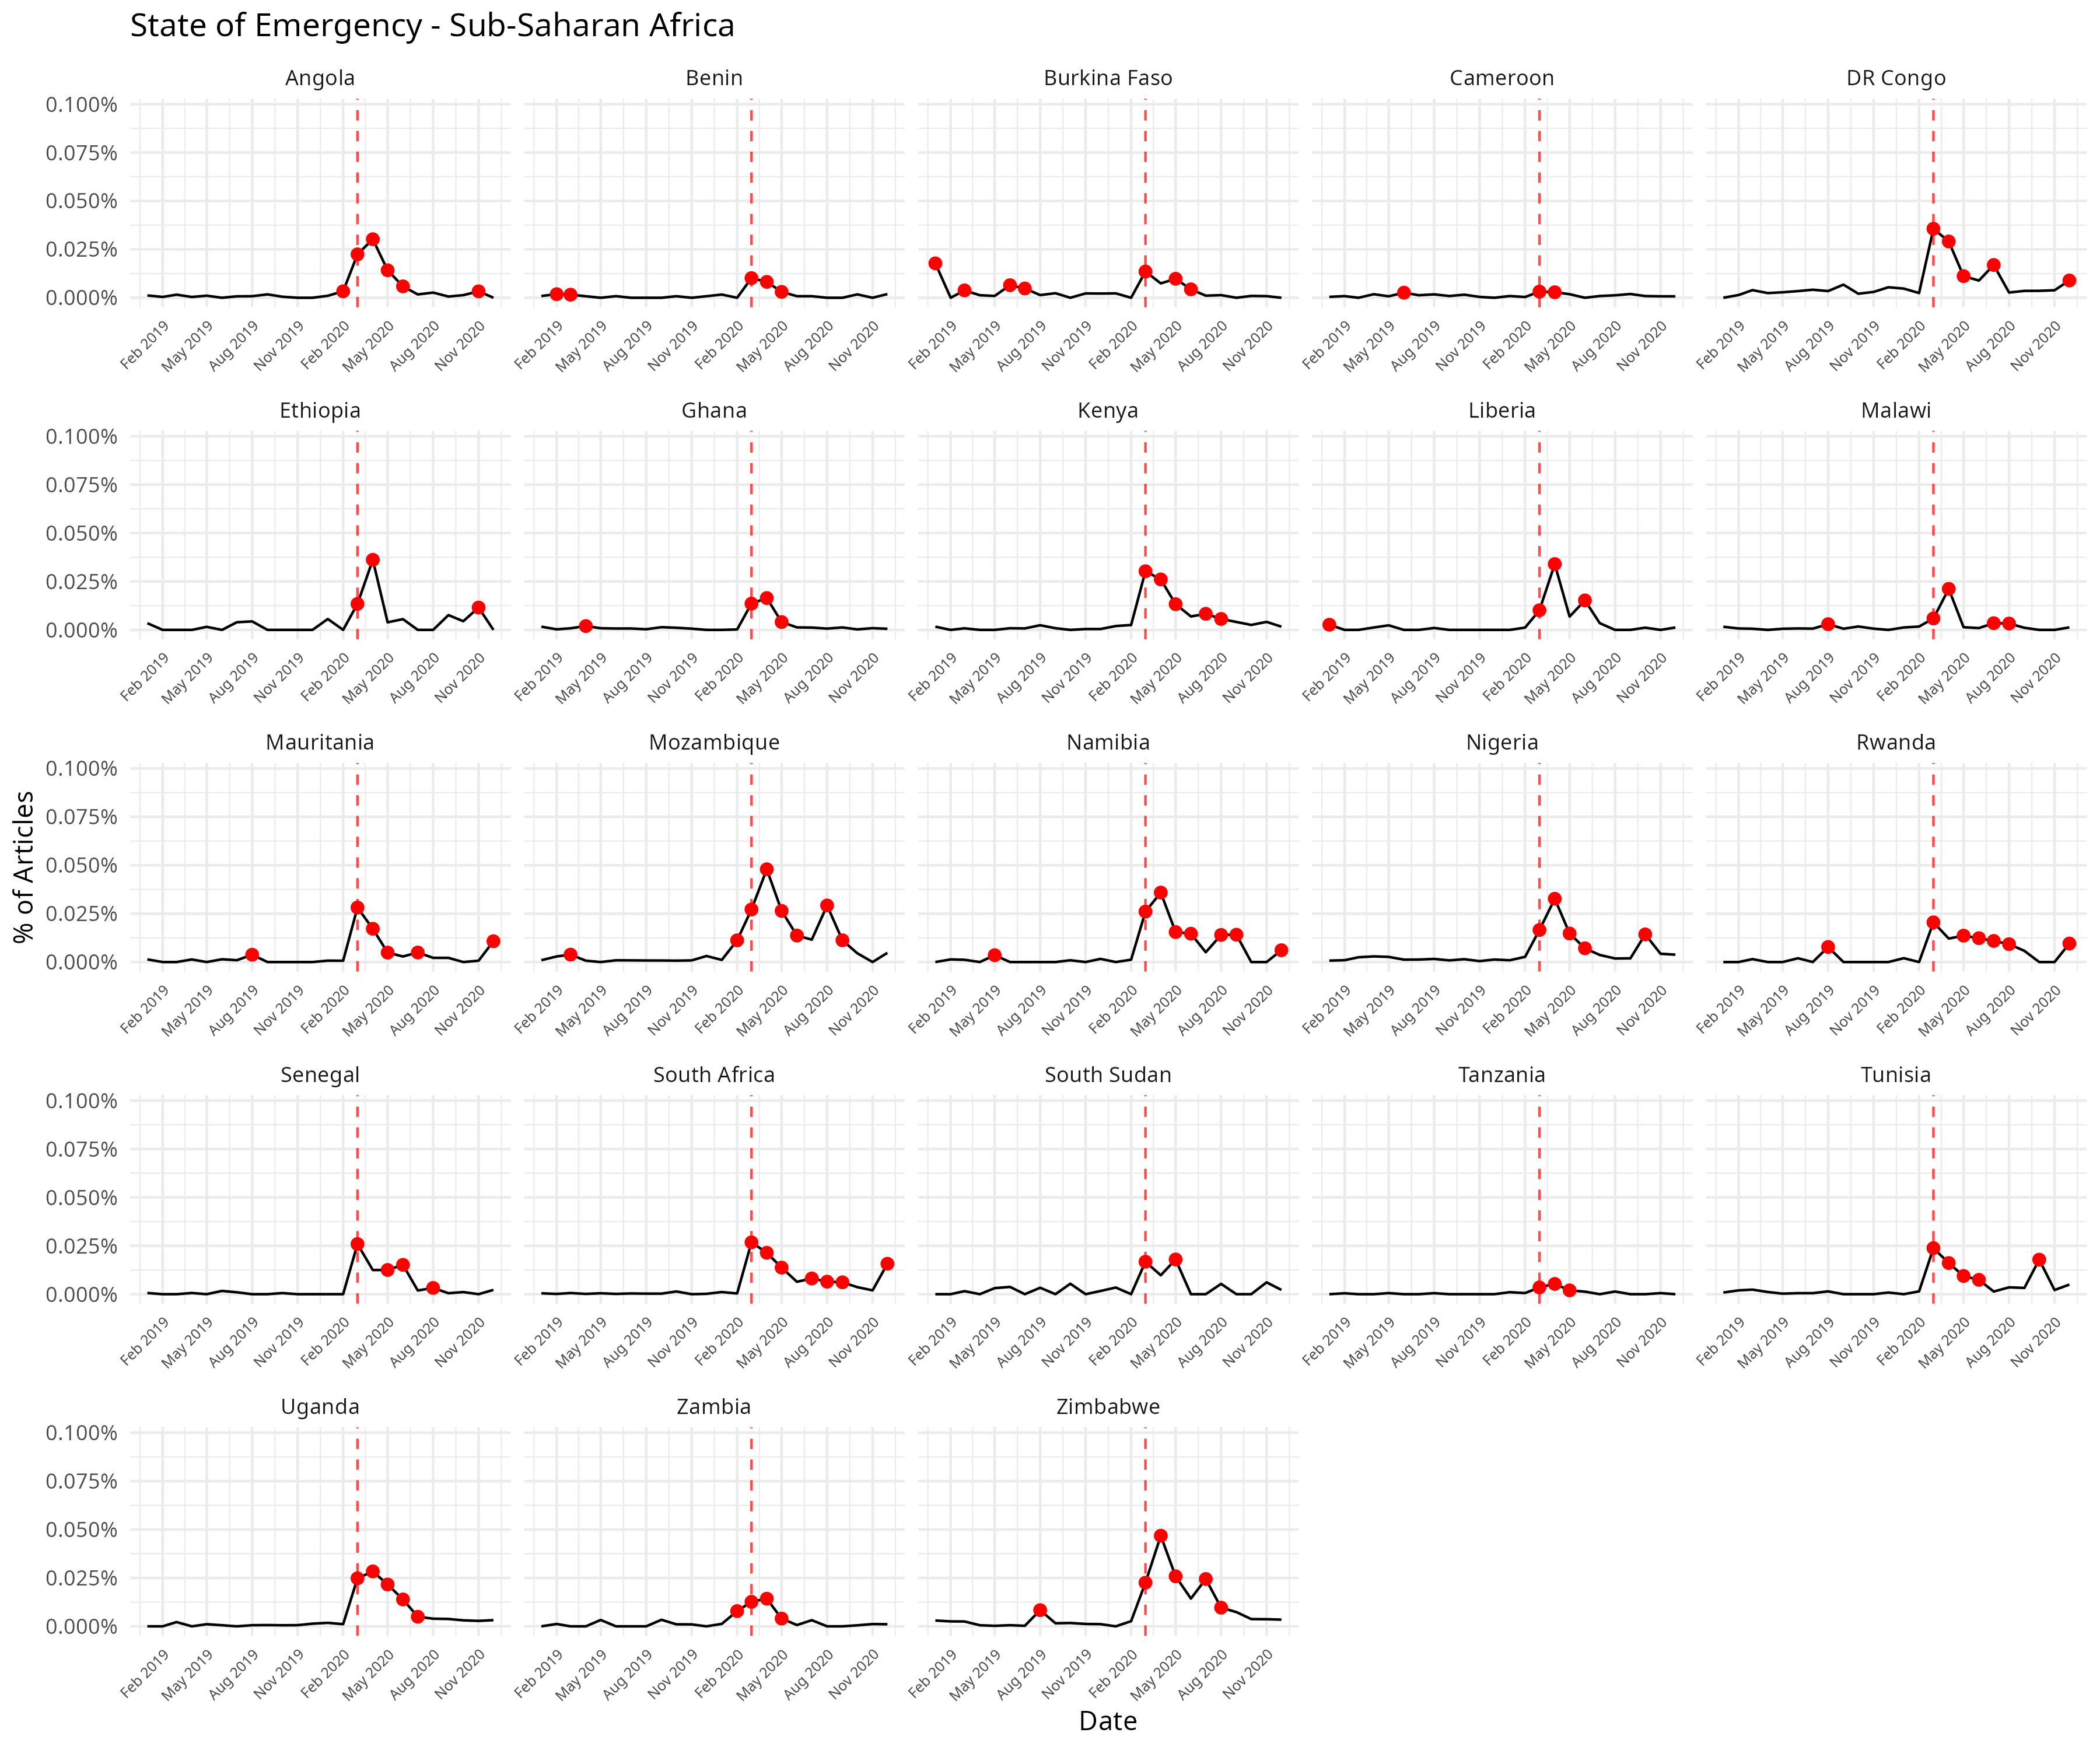
\includegraphics[width=1\linewidth,height=\textheight,keepaspectratio]{event_validation/State_of_Emergency_Sub-Saharan_Africa.png}
\# Appendix E: Detection of Civic Space Shocks

Our approach begins with winsorization of the monthlly normalized event
counts. This curbs the influence of extreme outliers by replacing values
beyond a specified percentile threshold with the nearest boundary value.
Next, we apply a 25-month rolling window to smooth the normalized event
counts and perform a grid search to tune various parameters. These
include the multipliers for weighted means and weighted standard
deviations, as well as the binning weights and decay functions that
govern how observations in the window are weighted. To capture shocks
accurately, we employ two distinct weighting schemes for the historical
(left-hand side, LHS) and future (right-hand side, RHS) segments of the
rolling window. For the LHS window, we use a non-linear decay weighting
that places progressively less emphasis on more distant historical
months, enabling the detection of rapid changes in recent data. For the
RHS window, we apply binning weights that decay linearly over time,
preventing overestimation of peaks when the underlying data structure
shifts. Combining winsorization with context-sensitive decay and binning
weights enables monthly detection of significant increases in each civic
space event type.

Next, we trained a neural network model to detect spikes in a
human-labeled dataset covering the full time-series for 30 country-event
pairs. We conducted human-labeling by asking humans to identify months
with visually distinct, sharp increases in our event measures. Human
labelers were instructed to identify no more than 15\% of overall months
as shocks, ensuring that peaks are not overly frequent in highly
variable data while still capturing meaningful shifts in lower-variance
event types. When either the statistical or neural network model detect
a shock, we label that month as a shock in the data.

\section{Appendix F: Event
Validation}\label{appendix-f-event-validation}

For each of the 40 country-event-month combinations, we retrieve all
relevant articles published by domestic outlets in the \emph{HQMARC}
corpus to determine whether these shocks are true or false positives.
Because some of these 40 country-event-months with shocks contained
hundreds of articles,\footnote{Across detected events, the number of
  relevant domestic articles ranged from 1 to 1,002. For rare event
  categories (e.g., \emph{Defamation Case}), a single article can define
  an event.} we used GPT-4o\footnote{The full GPT-4o prompts, GPT-4o
  generated summaries, human-coding instructions, and validation results
  can be found in the \texttt{shock-validation} subfolder of the Git
  repository. We accessed GPT-4o through the OpenAI API.} to generate
brief summaries of the five most important events reported on in the
sample of articles. A research assistant then reviewed both (a) the
original articles (or a random subset of 50, if more than 50 were
available) and (b) the GPT-4o summaries. They evaluated each of the top
five summarized events on four dimensions:

\begin{itemize}
\tightlist
\item
  How many summarized events are accurately described by GPT-4o (i.e.,
  factually correct)?
\item
  How many summarized events are indeed the most important events,
  according to the underlying articles?
\item
  How many occurred in the assigned country?
\item
  How many match the assigned event category?
\end{itemize}

\section{Appendix G: Forecasting Data and
Models}\label{appendix-g-forecasting-data-and-models}

Control variables include: a composite economic covariate calculated as
a within-country z-score of available monthly Trading Economics
indicators for each country. Given the importance of both gradual and
sudden shifts in political conditions, we lag all features by up to 12
months, allowing the model to detect both long-term precursors (such as
increasing government repression) and short-term triggers (such as
post-election violence). We account for persistence by including an
indicator distinguishing between new HLTA onsets and continued warnings,
a country-specific Bayesian prior that adjusts for baseline differences
in advisory issuance, and a COVID-19 indicator to control for the
pandemic-driven shock in travel warnings in 2020.

Results on our 6-month model yields a ROC-AUC of 0.87, AUC-PR of 0.31,
and a Brier score of 0.14 (dummy AUC-PR = 0.01), while the
rolling-window variant (±1 month) increases ROC-AUC to 0.90, AUC-PR to
0.57, and lowers the Brier score to 0.13, again with a dummy AUC-PR of
0.02.

Above and beyond these traditional measures of forecast accuracy, we
also trained the model on data through December 2023 and generated
predictions for advisory onsets in March and June 2024. The model
correctly flagged Bangladesh for June 2024, which later received an HLTA
due to the July Revolution. It also identified Zimbabwe and Liberia as
high-risk for March 2024, and while DOS did not issue an HLTA for these
countries, Zimbabwe expelled USAID staff in March, prompting U.S.
officials to issue multiple security statements. These cases highlight
the practical value of early warnings derived from high-frequency civic
space indicators, even when they do not always align with official
government actions.




\end{document}
